\documentclass[1p]{elsarticle_modified}
%\bibliographystyle{elsarticle-num}

%\usepackage[colorlinks]{hyperref}
%\usepackage{abbrmath_seonhwa} %\Abb, \Ascr, \Acal ,\Abf, \Afrak
\usepackage{amsfonts}
\usepackage{amssymb}
\usepackage{amsmath}
\usepackage{amsthm}
\usepackage{scalefnt}
\usepackage{amsbsy}
\usepackage{kotex}
\usepackage{caption}
\usepackage{subfig}
\usepackage{color}
\usepackage{graphicx}
\usepackage{xcolor} %% white, black, red, green, blue, cyan, magenta, yellow
\usepackage{float}
\usepackage{setspace}
\usepackage{hyperref}

\usepackage{tikz}
\usetikzlibrary{arrows}

\usepackage{multirow}
\usepackage{array} % fixed length table
\usepackage{hhline}

%%%%%%%%%%%%%%%%%%%%%
\makeatletter
\renewcommand*\env@matrix[1][\arraystretch]{%
	\edef\arraystretch{#1}%
	\hskip -\arraycolsep
	\let\@ifnextchar\new@ifnextchar
	\array{*\c@MaxMatrixCols c}}
\makeatother %https://tex.stackexchange.com/questions/14071/how-can-i-increase-the-line-spacing-in-a-matrix
%%%%%%%%%%%%%%%

\usepackage[normalem]{ulem}

\newcommand{\msout}[1]{\ifmmode\text{\sout{\ensuremath{#1}}}\else\sout{#1}\fi}
%SOURCE: \msout is \stkout macro in https://tex.stackexchange.com/questions/20609/strikeout-in-math-mode

\newcommand{\cancel}[1]{
	\ifmmode
	{\color{red}\msout{#1}}
	\else
	{\color{red}\sout{#1}}
	\fi
}

\newcommand{\add}[1]{
	{\color{blue}\uwave{#1}}
}

\newcommand{\replace}[2]{
	\ifmmode
	{\color{red}\msout{#1}}{\color{blue}\uwave{#2}}
	\else
	{\color{red}\sout{#1}}{\color{blue}\uwave{#2}}
	\fi
}

\newcommand{\Sol}{\mathcal{S}} %segment
\newcommand{\D}{D} %diagram
\newcommand{\A}{\mathcal{A}} %arc


%%%%%%%%%%%%%%%%%%%%%%%%%%%%%5 test

\def\sl{\operatorname{\textup{SL}}(2,\Cbb)}
\def\psl{\operatorname{\textup{PSL}}(2,\Cbb)}
\def\quan{\mkern 1mu \triangleright \mkern 1mu}

\theoremstyle{definition}
\newtheorem{thm}{Theorem}[section]
\newtheorem{prop}[thm]{Proposition}
\newtheorem{lem}[thm]{Lemma}
\newtheorem{ques}[thm]{Question}
\newtheorem{cor}[thm]{Corollary}
\newtheorem{defn}[thm]{Definition}
\newtheorem{exam}[thm]{Example}
\newtheorem{rmk}[thm]{Remark}
\newtheorem{alg}[thm]{Algorithm}

\newcommand{\I}{\sqrt{-1}}
\begin{document}

%\begin{frontmatter}
%
%\title{Boundary parabolic representations of knots up to 8 crossings}
%
%%% Group authors per affiliation:
%\author{Yunhi Cho} 
%\address{Department of Mathematics, University of Seoul, Seoul, Korea}
%\ead{yhcho@uos.ac.kr}
%
%
%\author{Seonhwa Kim} %\fnref{s_kim}}
%\address{Center for Geometry and Physics, Institute for Basic Science, Pohang, 37673, Korea}
%\ead{ryeona17@ibs.re.kr}
%
%\author{Hyuk Kim}
%\address{Department of Mathematical Sciences, Seoul National University, Seoul 08826, Korea}
%\ead{hyukkim@snu.ac.kr}
%
%\author{Seokbeom Yoon}
%\address{Department of Mathematical Sciences, Seoul National University, Seoul, 08826,  Korea}
%\ead{sbyoon15@snu.ac.kr}
%
%\begin{abstract}
%We find all boundary parabolic representation of knots up to 8 crossings.
%
%\end{abstract}
%\begin{keyword}
%    \MSC[2010] 57M25 
%\end{keyword}
%
%\end{frontmatter}

%\linenumbers
%\tableofcontents
%
\newcommand\colored[1]{\textcolor{white}{\rule[-0.35ex]{0.8em}{1.4ex}}\kern-0.8em\color{red} #1}%
%\newcommand\colored[1]{\textcolor{white}{ #1}\kern-2.17ex	\textcolor{white}{ #1}\kern-1.81ex	\textcolor{white}{ #1}\kern-2.15ex\color{red}#1	}

{\Large $\underline{12a_{0364}~(K12a_{0364})}$}

\setlength{\tabcolsep}{10pt}
\renewcommand{\arraystretch}{1.6}
\vspace{1cm}\begin{tabular}{m{100pt}>{\centering\arraybackslash}m{274pt}}
\multirow{5}{120pt}{
	\centering
	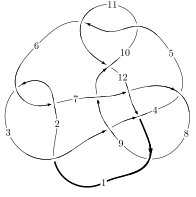
\includegraphics[width=112pt]{../../../GIT/diagram.site/Diagrams/png/1165_12a_0364.png}\\
\ \ \ A knot diagram\footnotemark}&
\allowdisplaybreaks
\textbf{Linearized knot diagam} \\
\cline{2-2}
 &
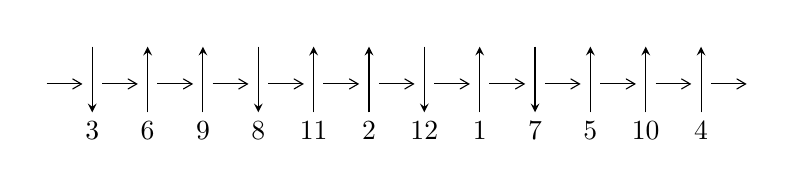
\begin{tikzpicture}[x=20pt, y=17pt]
	% nodes
	\node (C0) at (0, 0) {};
	\node (C1) at (1, 0) {};
	\node (C1U) at (1, +1) {};
	\node (C1D) at (1, -1) {3};

	\node (C2) at (2, 0) {};
	\node (C2U) at (2, +1) {};
	\node (C2D) at (2, -1) {6};

	\node (C3) at (3, 0) {};
	\node (C3U) at (3, +1) {};
	\node (C3D) at (3, -1) {9};

	\node (C4) at (4, 0) {};
	\node (C4U) at (4, +1) {};
	\node (C4D) at (4, -1) {8};

	\node (C5) at (5, 0) {};
	\node (C5U) at (5, +1) {};
	\node (C5D) at (5, -1) {11};

	\node (C6) at (6, 0) {};
	\node (C6U) at (6, +1) {};
	\node (C6D) at (6, -1) {2};

	\node (C7) at (7, 0) {};
	\node (C7U) at (7, +1) {};
	\node (C7D) at (7, -1) {12};

	\node (C8) at (8, 0) {};
	\node (C8U) at (8, +1) {};
	\node (C8D) at (8, -1) {1};

	\node (C9) at (9, 0) {};
	\node (C9U) at (9, +1) {};
	\node (C9D) at (9, -1) {7};

	\node (C10) at (10, 0) {};
	\node (C10U) at (10, +1) {};
	\node (C10D) at (10, -1) {5};

	\node (C11) at (11, 0) {};
	\node (C11U) at (11, +1) {};
	\node (C11D) at (11, -1) {10};

	\node (C12) at (12, 0) {};
	\node (C12U) at (12, +1) {};
	\node (C12D) at (12, -1) {4};
	\node (C13) at (13, 0) {};

	% arrows
	\draw[->,>={angle 60}]
	(C0) edge (C1) (C1) edge (C2) (C2) edge (C3) (C3) edge (C4) (C4) edge (C5) (C5) edge (C6) (C6) edge (C7) (C7) edge (C8) (C8) edge (C9) (C9) edge (C10) (C10) edge (C11) (C11) edge (C12) (C12) edge (C13) ;	\draw[->,>=stealth]
	(C1U) edge (C1D) (C2D) edge (C2U) (C3D) edge (C3U) (C4U) edge (C4D) (C5D) edge (C5U) (C6D) edge (C6U) (C7U) edge (C7D) (C8D) edge (C8U) (C9U) edge (C9D) (C10D) edge (C10U) (C11D) edge (C11U) (C12D) edge (C12U) ;
	\end{tikzpicture} \\
\hhline{~~} \\& 
\textbf{Solving Sequence} \\ \cline{2-2} 
 &
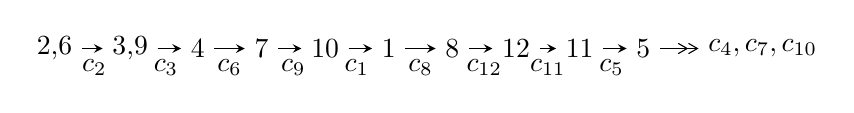
\begin{tikzpicture}[x=23pt, y=7pt]
	% node
	\node (A0) at (-1/8, 0) {2,6};
	\node (A1) at (17/16, 0) {3,9};
	\node (A2) at (17/8, 0) {4};
	\node (A3) at (25/8, 0) {7};
	\node (A4) at (33/8, 0) {10};
	\node (A5) at (41/8, 0) {1};
	\node (A6) at (49/8, 0) {8};
	\node (A7) at (57/8, 0) {12};
	\node (A8) at (65/8, 0) {11};
	\node (A9) at (73/8, 0) {5};
	\node (C1) at (1/2, -1) {$c_{2}$};
	\node (C2) at (13/8, -1) {$c_{3}$};
	\node (C3) at (21/8, -1) {$c_{6}$};
	\node (C4) at (29/8, -1) {$c_{9}$};
	\node (C5) at (37/8, -1) {$c_{1}$};
	\node (C6) at (45/8, -1) {$c_{8}$};
	\node (C7) at (53/8, -1) {$c_{12}$};
	\node (C8) at (61/8, -1) {$c_{11}$};
	\node (C9) at (69/8, -1) {$c_{5}$};
	\node (A10) at (11, 0) {$c_{4},c_{7},c_{10}$};

	% edge
	\draw[->,>=stealth]	
	(A0) edge (A1) (A1) edge (A2) (A2) edge (A3) (A3) edge (A4) (A4) edge (A5) (A5) edge (A6) (A6) edge (A7) (A7) edge (A8) (A8) edge (A9) ;
	\draw[->>,>={angle 60}]	
	(A9) edge (A10);
\end{tikzpicture} \\ 

\end{tabular} \\

\footnotetext{
The image of knot diagram is generated by the software ``\textbf{Draw programme}" developed by Andrew Bartholomew(\url{http://www.layer8.co.uk/maths/draw/index.htm\#Running-draw}), where we modified some parts for our purpose(\url{https://github.com/CATsTAILs/LinksPainter}).
}\phantom \\ \newline 
\centering \textbf{Ideals for irreducible components\footnotemark of $X_{\text{par}}$} 
 
\begin{align*}
I^u_{1}&=\langle 
3.06101\times10^{668} u^{182}+1.45399\times10^{669} u^{181}+\cdots+3.50750\times10^{668} b+1.63631\times10^{672},\\
\phantom{I^u_{1}}&\phantom{= \langle  }-4.31223\times10^{671} u^{182}+1.20316\times10^{672} u^{181}+\cdots+3.97400\times10^{671} a+1.18875\times10^{675},\\
\phantom{I^u_{1}}&\phantom{= \langle  }u^{183}+u^{182}+\cdots+4256 u+1133\rangle \\
I^u_{2}&=\langle 
24823104 u^{41}-19103471 u^{40}+\cdots+3944339 b-19426104,\\
\phantom{I^u_{2}}&\phantom{= \langle  }10847937 u^{41}-23370443 u^{40}+\cdots+3944339 a+1833879,\;u^{42}+11 u^{40}+\cdots- u+1\rangle \\
\\
\end{align*}
\raggedright * 2 irreducible components of $\dim_{\mathbb{C}}=0$, with total 225 representations.\\
\footnotetext{All coefficients of polynomials are rational numbers. But the coefficients are sometimes approximated in decimal forms when there is not enough margin.}
\newpage
\renewcommand{\arraystretch}{1}
\centering \section*{I. $I^u_{1}= \langle 3.06\times10^{668} u^{182}+1.45\times10^{669} u^{181}+\cdots+3.51\times10^{668} b+1.64\times10^{672},\;-4.31\times10^{671} u^{182}+1.20\times10^{672} u^{181}+\cdots+3.97\times10^{671} a+1.19\times10^{675},\;u^{183}+u^{182}+\cdots+4256 u+1133 \rangle$}
\flushleft \textbf{(i) Arc colorings}\\
\begin{tabular}{m{7pt} m{180pt} m{7pt} m{180pt} }
\flushright $a_{2}=$&$\begin{pmatrix}1\\0\end{pmatrix}$ \\
\flushright $a_{6}=$&$\begin{pmatrix}0\\u\end{pmatrix}$ \\
\flushright $a_{3}=$&$\begin{pmatrix}1\\- u^2\end{pmatrix}$ \\
\flushright $a_{9}=$&$\begin{pmatrix}1.08511 u^{182}-3.02757 u^{181}+\cdots-7046.61 u-2991.31\\-0.872703 u^{182}-4.14537 u^{181}+\cdots-13315.2 u-4665.18\end{pmatrix}$ \\
\flushright $a_{4}=$&$\begin{pmatrix}1.12129 u^{182}+0.925627 u^{181}+\cdots+4093.75 u+1132.16\\1.05786 u^{182}+1.82765 u^{181}+\cdots+6881.98 u+2201.09\end{pmatrix}$ \\
\flushright $a_{7}=$&$\begin{pmatrix}u\\u\end{pmatrix}$ \\
\flushright $a_{10}=$&$\begin{pmatrix}-0.139695 u^{182}-1.77491 u^{181}+\cdots-5689.73 u-2039.58\\-2.09751 u^{182}-2.89272 u^{181}+\cdots-11958.4 u-3713.44\end{pmatrix}$ \\
\flushright $a_{1}=$&$\begin{pmatrix}u^2+1\\- u^4\end{pmatrix}$ \\
\flushright $a_{8}=$&$\begin{pmatrix}-0.320040 u^{182}-2.23656 u^{181}+\cdots-7280.85 u-2535.00\\-1.70018 u^{182}-2.74137 u^{181}+\cdots-10716.3 u-3390.53\end{pmatrix}$ \\
\flushright $a_{12}=$&$\begin{pmatrix}-0.323583 u^{182}-0.355194 u^{181}+\cdots-1218.60 u-260.576\\-2.31378 u^{182}-1.07817 u^{181}+\cdots-5843.16 u-1298.01\end{pmatrix}$ \\
\flushright $a_{11}=$&$\begin{pmatrix}-0.0734871 u^{182}+2.24058 u^{181}+\cdots+6864.55 u+2639.36\\-3.39552 u^{182}+1.13443 u^{181}+\cdots-496.042 u+1175.34\end{pmatrix}$ \\
\flushright $a_{5}=$&$\begin{pmatrix}1.99923 u^{182}+1.23701 u^{181}+\cdots+6552.84 u+1660.68\\1.79503 u^{182}-4.25068 u^{181}+\cdots-10911.1 u-4668.15\end{pmatrix}$\\&\end{tabular}
\flushleft \textbf{(ii) Obstruction class $= -1$}\\~\\
\flushleft \textbf{(iii) Cusp Shapes $= 1.45862 u^{182}+0.408690 u^{181}+\cdots+1561.89 u+128.705$}\\~\\
\newpage\renewcommand{\arraystretch}{1}
\flushleft \textbf{(iv) u-Polynomials at the component}\newline \\
\begin{tabular}{m{50pt}|m{274pt}}
Crossings & \hspace{64pt}u-Polynomials at each crossing \\
\hline $$\begin{aligned}c_{1}\end{aligned}$$&$\begin{aligned}
&u^{183}+77 u^{182}+\cdots-46277120 u-1283689
\end{aligned}$\\
\hline $$\begin{aligned}c_{2},c_{6}\end{aligned}$$&$\begin{aligned}
&u^{183}- u^{182}+\cdots+4256 u-1133
\end{aligned}$\\
\hline $$\begin{aligned}c_{3}\end{aligned}$$&$\begin{aligned}
&u^{183}+u^{182}+\cdots+31 u-3
\end{aligned}$\\
\hline $$\begin{aligned}c_{4}\end{aligned}$$&$\begin{aligned}
&u^{183}+3 u^{182}+\cdots+555350 u-53533
\end{aligned}$\\
\hline $$\begin{aligned}c_{5},c_{10}\end{aligned}$$&$\begin{aligned}
&u^{183}+u^{182}+\cdots-173 u-59
\end{aligned}$\\
\hline $$\begin{aligned}c_{7}\end{aligned}$$&$\begin{aligned}
&u^{183}-2 u^{182}+\cdots+334697 u-27379
\end{aligned}$\\
\hline $$\begin{aligned}c_{8}\end{aligned}$$&$\begin{aligned}
&u^{183}-5 u^{182}+\cdots-6926 u-485
\end{aligned}$\\
\hline $$\begin{aligned}c_{9}\end{aligned}$$&$\begin{aligned}
&u^{183}+7 u^{182}+\cdots+1157925 u-194803
\end{aligned}$\\
\hline $$\begin{aligned}c_{11}\end{aligned}$$&$\begin{aligned}
&u^{183}-87 u^{182}+\cdots+82911 u-3481
\end{aligned}$\\
\hline $$\begin{aligned}c_{12}\end{aligned}$$&$\begin{aligned}
&u^{183}+16 u^{182}+\cdots-199 u-7
\end{aligned}$\\
\hline
\end{tabular}\\~\\
\newpage\renewcommand{\arraystretch}{1}
\flushleft \textbf{(v) Riley Polynomials at the component}\newline \\
\begin{tabular}{m{50pt}|m{274pt}}
Crossings & \hspace{64pt}Riley Polynomials at each crossing \\
\hline $$\begin{aligned}c_{1}\end{aligned}$$&$\begin{aligned}
&y^{183}+65 y^{182}+\cdots-180776219221564 y-1647857448721
\end{aligned}$\\
\hline $$\begin{aligned}c_{2},c_{6}\end{aligned}$$&$\begin{aligned}
&y^{183}+77 y^{182}+\cdots-46277120 y-1283689
\end{aligned}$\\
\hline $$\begin{aligned}c_{3}\end{aligned}$$&$\begin{aligned}
&y^{183}-17 y^{182}+\cdots+67 y-9
\end{aligned}$\\
\hline $$\begin{aligned}c_{4}\end{aligned}$$&$\begin{aligned}
&y^{183}+11 y^{182}+\cdots-122436449664 y-2865782089
\end{aligned}$\\
\hline $$\begin{aligned}c_{5},c_{10}\end{aligned}$$&$\begin{aligned}
&y^{183}-87 y^{182}+\cdots+82911 y-3481
\end{aligned}$\\
\hline $$\begin{aligned}c_{7}\end{aligned}$$&$\begin{aligned}
&y^{183}-28 y^{182}+\cdots-2771494231 y-749609641
\end{aligned}$\\
\hline $$\begin{aligned}c_{8}\end{aligned}$$&$\begin{aligned}
&y^{183}-29 y^{182}+\cdots-40132714 y-235225
\end{aligned}$\\
\hline $$\begin{aligned}c_{9}\end{aligned}$$&$\begin{aligned}
&y^{183}-11 y^{182}+\cdots-18463850066073 y-37948208809
\end{aligned}$\\
\hline $$\begin{aligned}c_{11}\end{aligned}$$&$\begin{aligned}
&y^{183}+33 y^{182}+\cdots+364826579 y-12117361
\end{aligned}$\\
\hline $$\begin{aligned}c_{12}\end{aligned}$$&$\begin{aligned}
&y^{183}+10 y^{182}+\cdots-2819 y-49
\end{aligned}$\\
\hline
\end{tabular}\\~\\
\newpage\flushleft \textbf{(vi) Complex Volumes and Cusp Shapes}
$$\begin{array}{c|c|c}  
\text{Solutions to }I^u_{1}& \I (\text{vol} + \sqrt{-1}CS) & \text{Cusp shape}\\
 \hline 
\begin{aligned}
u &= \phantom{-}0.002506 + 1.001090 I \\
a &= -0.301136 + 1.067720 I \\
b &= \phantom{-}0.015541 + 0.450831 I\end{aligned}
 & -2.35185 - 1.36074 I & \phantom{-0.000000 } 0 \\ \hline\begin{aligned}
u &= \phantom{-}0.002506 - 1.001090 I \\
a &= -0.301136 - 1.067720 I \\
b &= \phantom{-}0.015541 - 0.450831 I\end{aligned}
 & -2.35185 + 1.36074 I & \phantom{-0.000000 } 0 \\ \hline\begin{aligned}
u &= \phantom{-}0.657408 + 0.760366 I \\
a &= \phantom{-}0.640158 - 0.397181 I \\
b &= -0.0807366 + 0.0498924 I\end{aligned}
 & \phantom{-}3.94780 - 1.03684 I & \phantom{-0.000000 } 0 \\ \hline\begin{aligned}
u &= \phantom{-}0.657408 - 0.760366 I \\
a &= \phantom{-}0.640158 + 0.397181 I \\
b &= -0.0807366 - 0.0498924 I\end{aligned}
 & \phantom{-}3.94780 + 1.03684 I & \phantom{-0.000000 } 0 \\ \hline\begin{aligned}
u &= -0.907481 + 0.395088 I \\
a &= -0.975120 - 0.368474 I \\
b &= -0.023349 - 0.616263 I\end{aligned}
 & \phantom{-}1.78380 + 1.10430 I & \phantom{-0.000000 } 0 \\ \hline\begin{aligned}
u &= -0.907481 - 0.395088 I \\
a &= -0.975120 + 0.368474 I \\
b &= -0.023349 + 0.616263 I\end{aligned}
 & \phantom{-}1.78380 - 1.10430 I & \phantom{-0.000000 } 0 \\ \hline\begin{aligned}
u &= -0.346743 + 0.922544 I \\
a &= -1.94060 + 0.03413 I \\
b &= -2.05091 - 0.63156 I\end{aligned}
 & -2.22716 + 1.66256 I & \phantom{-0.000000 } 0 \\ \hline\begin{aligned}
u &= -0.346743 - 0.922544 I \\
a &= -1.94060 - 0.03413 I \\
b &= -2.05091 + 0.63156 I\end{aligned}
 & -2.22716 - 1.66256 I & \phantom{-0.000000 } 0 \\ \hline\begin{aligned}
u &= -0.832406 + 0.580904 I \\
a &= -0.816072 - 1.107820 I \\
b &= \phantom{-}0.21102 - 1.46237 I\end{aligned}
 & \phantom{-}5.69571 + 6.18009 I & \phantom{-0.000000 } 0 \\ \hline\begin{aligned}
u &= -0.832406 - 0.580904 I \\
a &= -0.816072 + 1.107820 I \\
b &= \phantom{-}0.21102 + 1.46237 I\end{aligned}
 & \phantom{-}5.69571 - 6.18009 I & \phantom{-0.000000 } 0\\
 \hline 
 \end{array}$$\newpage$$\begin{array}{c|c|c}  
\text{Solutions to }I^u_{1}& \I (\text{vol} + \sqrt{-1}CS) & \text{Cusp shape}\\
 \hline 
\begin{aligned}
u &= \phantom{-}0.445854 + 0.912506 I \\
a &= -0.250178 + 0.647036 I \\
b &= \phantom{-}0.582212 - 0.638228 I\end{aligned}
 & -4.07840 + 1.74509 I & \phantom{-0.000000 } 0 \\ \hline\begin{aligned}
u &= \phantom{-}0.445854 - 0.912506 I \\
a &= -0.250178 - 0.647036 I \\
b &= \phantom{-}0.582212 + 0.638228 I\end{aligned}
 & -4.07840 - 1.74509 I & \phantom{-0.000000 } 0 \\ \hline\begin{aligned}
u &= -0.550473 + 0.855625 I \\
a &= \phantom{-}1.58869 + 0.29474 I \\
b &= \phantom{-}1.47188 + 2.18116 I\end{aligned}
 & \phantom{-}3.11251 - 0.85633 I & \phantom{-0.000000 } 0 \\ \hline\begin{aligned}
u &= -0.550473 - 0.855625 I \\
a &= \phantom{-}1.58869 - 0.29474 I \\
b &= \phantom{-}1.47188 - 2.18116 I\end{aligned}
 & \phantom{-}3.11251 + 0.85633 I & \phantom{-0.000000 } 0 \\ \hline\begin{aligned}
u &= -0.550724 + 0.859621 I \\
a &= -1.54212 - 1.93111 I \\
b &= \phantom{-}0.40476 - 1.59933 I\end{aligned}
 & \phantom{-}3.09891 - 3.55549 I & \phantom{-0.000000 } 0 \\ \hline\begin{aligned}
u &= -0.550724 - 0.859621 I \\
a &= -1.54212 + 1.93111 I \\
b &= \phantom{-}0.40476 + 1.59933 I\end{aligned}
 & \phantom{-}3.09891 + 3.55549 I & \phantom{-0.000000 } 0 \\ \hline\begin{aligned}
u &= \phantom{-}0.539399 + 0.794949 I \\
a &= \phantom{-}1.32069 - 1.68704 I \\
b &= \phantom{-}1.17697 - 2.20251 I\end{aligned}
 & \phantom{-}6.50793 + 1.54821 I & \phantom{-0.000000 } 0 \\ \hline\begin{aligned}
u &= \phantom{-}0.539399 - 0.794949 I \\
a &= \phantom{-}1.32069 + 1.68704 I \\
b &= \phantom{-}1.17697 + 2.20251 I\end{aligned}
 & \phantom{-}6.50793 - 1.54821 I & \phantom{-0.000000 } 0 \\ \hline\begin{aligned}
u &= -0.100235 + 1.035900 I \\
a &= \phantom{-}0.418216 + 0.328869 I \\
b &= -0.218597 - 1.065900 I\end{aligned}
 & -6.21715 - 0.49274 I & \phantom{-0.000000 } 0 \\ \hline\begin{aligned}
u &= -0.100235 - 1.035900 I \\
a &= \phantom{-}0.418216 - 0.328869 I \\
b &= -0.218597 + 1.065900 I\end{aligned}
 & -6.21715 + 0.49274 I & \phantom{-0.000000 } 0\\
 \hline 
 \end{array}$$\newpage$$\begin{array}{c|c|c}  
\text{Solutions to }I^u_{1}& \I (\text{vol} + \sqrt{-1}CS) & \text{Cusp shape}\\
 \hline 
\begin{aligned}
u &= \phantom{-}0.747476 + 0.729954 I \\
a &= -1.42324 + 0.66409 I \\
b &= -0.32911 + 2.22620 I\end{aligned}
 & \phantom{-}2.50612 - 1.04846 I & \phantom{-0.000000 } 0 \\ \hline\begin{aligned}
u &= \phantom{-}0.747476 - 0.729954 I \\
a &= -1.42324 - 0.66409 I \\
b &= -0.32911 - 2.22620 I\end{aligned}
 & \phantom{-}2.50612 + 1.04846 I & \phantom{-0.000000 } 0 \\ \hline\begin{aligned}
u &= -0.557270 + 0.773086 I \\
a &= \phantom{-}2.28692 + 1.27034 I \\
b &= \phantom{-}1.14776 + 1.11615 I\end{aligned}
 & -0.232614 + 0.596001 I & \phantom{-0.000000 } 0 \\ \hline\begin{aligned}
u &= -0.557270 - 0.773086 I \\
a &= \phantom{-}2.28692 - 1.27034 I \\
b &= \phantom{-}1.14776 - 1.11615 I\end{aligned}
 & -0.232614 - 0.596001 I & \phantom{-0.000000 } 0 \\ \hline\begin{aligned}
u &= \phantom{-}0.627455 + 0.716670 I \\
a &= -2.33890 + 0.93316 I \\
b &= -0.807083 + 1.028980 I\end{aligned}
 & \phantom{-}2.26284 - 6.40383 I & \phantom{-0.000000 } 0 \\ \hline\begin{aligned}
u &= \phantom{-}0.627455 - 0.716670 I \\
a &= -2.33890 - 0.93316 I \\
b &= -0.807083 - 1.028980 I\end{aligned}
 & \phantom{-}2.26284 + 6.40383 I & \phantom{-0.000000 } 0 \\ \hline\begin{aligned}
u &= \phantom{-}0.728434 + 0.611027 I \\
a &= \phantom{-}1.24633 - 0.73003 I \\
b &= \phantom{-}0.482467 - 1.183330 I\end{aligned}
 & \phantom{-}7.15615 + 1.84565 I & \phantom{-0.000000 } 0 \\ \hline\begin{aligned}
u &= \phantom{-}0.728434 - 0.611027 I \\
a &= \phantom{-}1.24633 + 0.73003 I \\
b &= \phantom{-}0.482467 + 1.183330 I\end{aligned}
 & \phantom{-}7.15615 - 1.84565 I & \phantom{-0.000000 } 0 \\ \hline\begin{aligned}
u &= \phantom{-}0.433567 + 0.963298 I \\
a &= \phantom{-}1.84915 - 0.03503 I \\
b &= \phantom{-}1.84761 - 1.03237 I\end{aligned}
 & -3.99443 + 3.51059 I & \phantom{-0.000000 } 0 \\ \hline\begin{aligned}
u &= \phantom{-}0.433567 - 0.963298 I \\
a &= \phantom{-}1.84915 + 0.03503 I \\
b &= \phantom{-}1.84761 + 1.03237 I\end{aligned}
 & -3.99443 - 3.51059 I & \phantom{-0.000000 } 0\\
 \hline 
 \end{array}$$\newpage$$\begin{array}{c|c|c}  
\text{Solutions to }I^u_{1}& \I (\text{vol} + \sqrt{-1}CS) & \text{Cusp shape}\\
 \hline 
\begin{aligned}
u &= \phantom{-}0.931814 + 0.508864 I \\
a &= \phantom{-}0.913621 - 1.050700 I \\
b &= -0.474141 - 1.264530 I\end{aligned}
 & -0.02127 - 9.16097 I & \phantom{-0.000000 } 0 \\ \hline\begin{aligned}
u &= \phantom{-}0.931814 - 0.508864 I \\
a &= \phantom{-}0.913621 + 1.050700 I \\
b &= -0.474141 + 1.264530 I\end{aligned}
 & -0.02127 + 9.16097 I & \phantom{-0.000000 } 0 \\ \hline\begin{aligned}
u &= -0.986706 + 0.407027 I \\
a &= \phantom{-}0.636220 + 0.399246 I \\
b &= -0.065403 + 0.890735 I\end{aligned}
 & \phantom{-}4.94639 + 5.58121 I & \phantom{-0.000000 } 0 \\ \hline\begin{aligned}
u &= -0.986706 - 0.407027 I \\
a &= \phantom{-}0.636220 - 0.399246 I \\
b &= -0.065403 - 0.890735 I\end{aligned}
 & \phantom{-}4.94639 - 5.58121 I & \phantom{-0.000000 } 0 \\ \hline\begin{aligned}
u &= -0.654680 + 0.844531 I \\
a &= -1.20925 + 0.95465 I \\
b &= -1.196920 + 0.684125 I\end{aligned}
 & \phantom{-}0.61558 - 2.54624 I & \phantom{-0.000000 } 0 \\ \hline\begin{aligned}
u &= -0.654680 - 0.844531 I \\
a &= -1.20925 - 0.95465 I \\
b &= -1.196920 - 0.684125 I\end{aligned}
 & \phantom{-}0.61558 + 2.54624 I & \phantom{-0.000000 } 0 \\ \hline\begin{aligned}
u &= \phantom{-}0.731449 + 0.571623 I \\
a &= -1.53574 + 1.48199 I \\
b &= \phantom{-}0.37856 + 1.76760 I\end{aligned}
 & -0.37741 - 5.71633 I & \phantom{-0.000000 } 0 \\ \hline\begin{aligned}
u &= \phantom{-}0.731449 - 0.571623 I \\
a &= -1.53574 - 1.48199 I \\
b &= \phantom{-}0.37856 - 1.76760 I\end{aligned}
 & -0.37741 + 5.71633 I & \phantom{-0.000000 } 0 \\ \hline\begin{aligned}
u &= -0.516145 + 0.771156 I \\
a &= \phantom{-}0.952646 + 0.811885 I \\
b &= -0.324158 - 0.327902 I\end{aligned}
 & -0.53621 + 2.32801 I & \phantom{-0.000000 } 0 \\ \hline\begin{aligned}
u &= -0.516145 - 0.771156 I \\
a &= \phantom{-}0.952646 - 0.811885 I \\
b &= -0.324158 + 0.327902 I\end{aligned}
 & -0.53621 - 2.32801 I & \phantom{-0.000000 } 0\\
 \hline 
 \end{array}$$\newpage$$\begin{array}{c|c|c}  
\text{Solutions to }I^u_{1}& \I (\text{vol} + \sqrt{-1}CS) & \text{Cusp shape}\\
 \hline 
\begin{aligned}
u &= \phantom{-}0.926464 + 0.046019 I \\
a &= -0.367772 - 0.284571 I \\
b &= -0.358099 - 0.222420 I\end{aligned}
 & \phantom{-}3.54138 + 2.83842 I & \phantom{-0.000000 } 0 \\ \hline\begin{aligned}
u &= \phantom{-}0.926464 - 0.046019 I \\
a &= -0.367772 + 0.284571 I \\
b &= -0.358099 + 0.222420 I\end{aligned}
 & \phantom{-}3.54138 - 2.83842 I & \phantom{-0.000000 } 0 \\ \hline\begin{aligned}
u &= \phantom{-}0.012896 + 1.073490 I \\
a &= -0.737068 - 0.531654 I \\
b &= -0.405083 + 0.417015 I\end{aligned}
 & -0.32963 + 5.18055 I & \phantom{-0.000000 } 0 \\ \hline\begin{aligned}
u &= \phantom{-}0.012896 - 1.073490 I \\
a &= -0.737068 + 0.531654 I \\
b &= -0.405083 - 0.417015 I\end{aligned}
 & -0.32963 - 5.18055 I & \phantom{-0.000000 } 0 \\ \hline\begin{aligned}
u &= -0.568689 + 0.915928 I \\
a &= -0.82583 - 1.67184 I \\
b &= -0.74892 - 2.67127 I\end{aligned}
 & -0.69467 - 5.11406 I & \phantom{-0.000000 } 0 \\ \hline\begin{aligned}
u &= -0.568689 - 0.915928 I \\
a &= -0.82583 + 1.67184 I \\
b &= -0.74892 + 2.67127 I\end{aligned}
 & -0.69467 + 5.11406 I & \phantom{-0.000000 } 0 \\ \hline\begin{aligned}
u &= \phantom{-}0.619160 + 0.882815 I \\
a &= -0.462784 - 0.132943 I \\
b &= -1.094350 + 0.862174 I\end{aligned}
 & \phantom{-}3.61626 + 6.02592 I & \phantom{-0.000000 } 0 \\ \hline\begin{aligned}
u &= \phantom{-}0.619160 - 0.882815 I \\
a &= -0.462784 + 0.132943 I \\
b &= -1.094350 - 0.862174 I\end{aligned}
 & \phantom{-}3.61626 - 6.02592 I & \phantom{-0.000000 } 0 \\ \hline\begin{aligned}
u &= -0.543038 + 0.933500 I \\
a &= \phantom{-}0.257256 + 0.203403 I \\
b &= -0.434241 - 0.990715 I\end{aligned}
 & -1.09057 - 6.62662 I & \phantom{-0.000000 } 0 \\ \hline\begin{aligned}
u &= -0.543038 - 0.933500 I \\
a &= \phantom{-}0.257256 - 0.203403 I \\
b &= -0.434241 + 0.990715 I\end{aligned}
 & -1.09057 + 6.62662 I & \phantom{-0.000000 } 0\\
 \hline 
 \end{array}$$\newpage$$\begin{array}{c|c|c}  
\text{Solutions to }I^u_{1}& \I (\text{vol} + \sqrt{-1}CS) & \text{Cusp shape}\\
 \hline 
\begin{aligned}
u &= -0.707658 + 0.818823 I \\
a &= \phantom{-}1.55822 + 0.50718 I \\
b &= \phantom{-}0.78450 + 2.51756 I\end{aligned}
 & \phantom{-}3.25753 + 4.56073 I & \phantom{-0.000000 } 0 \\ \hline\begin{aligned}
u &= -0.707658 - 0.818823 I \\
a &= \phantom{-}1.55822 - 0.50718 I \\
b &= \phantom{-}0.78450 - 2.51756 I\end{aligned}
 & \phantom{-}3.25753 - 4.56073 I & \phantom{-0.000000 } 0 \\ \hline\begin{aligned}
u &= \phantom{-}0.757720 + 0.507649 I \\
a &= -0.865308 + 0.335743 I \\
b &= -0.357419 + 1.226330 I\end{aligned}
 & \phantom{-}2.79108 - 2.17795 I & \phantom{-0.000000 } 0 \\ \hline\begin{aligned}
u &= \phantom{-}0.757720 - 0.507649 I \\
a &= -0.865308 - 0.335743 I \\
b &= -0.357419 - 1.226330 I\end{aligned}
 & \phantom{-}2.79108 + 2.17795 I & \phantom{-0.000000 } 0 \\ \hline\begin{aligned}
u &= -0.765290 + 0.777732 I \\
a &= \phantom{-}0.313788 - 0.283363 I \\
b &= \phantom{-}0.764073 + 0.447255 I\end{aligned}
 & \phantom{-}1.24383 - 2.75337 I & \phantom{-0.000000 } 0 \\ \hline\begin{aligned}
u &= -0.765290 - 0.777732 I \\
a &= \phantom{-}0.313788 + 0.283363 I \\
b &= \phantom{-}0.764073 - 0.447255 I\end{aligned}
 & \phantom{-}1.24383 + 2.75337 I & \phantom{-0.000000 } 0 \\ \hline\begin{aligned}
u &= -0.642154 + 0.885034 I \\
a &= -0.605908 - 0.137387 I \\
b &= -0.1325530 - 0.0361140 I\end{aligned}
 & \phantom{-}0.97256 - 2.56913 I & \phantom{-0.000000 } 0 \\ \hline\begin{aligned}
u &= -0.642154 - 0.885034 I \\
a &= -0.605908 + 0.137387 I \\
b &= -0.1325530 + 0.0361140 I\end{aligned}
 & \phantom{-}0.97256 + 2.56913 I & \phantom{-0.000000 } 0 \\ \hline\begin{aligned}
u &= \phantom{-}0.595783 + 0.918335 I \\
a &= -1.67611 + 1.20857 I \\
b &= -1.09082 + 1.56018 I\end{aligned}
 & \phantom{-}6.04330 + 2.97947 I & \phantom{-0.000000 } 0 \\ \hline\begin{aligned}
u &= \phantom{-}0.595783 - 0.918335 I \\
a &= -1.67611 - 1.20857 I \\
b &= -1.09082 - 1.56018 I\end{aligned}
 & \phantom{-}6.04330 - 2.97947 I & \phantom{-0.000000 } 0\\
 \hline 
 \end{array}$$\newpage$$\begin{array}{c|c|c}  
\text{Solutions to }I^u_{1}& \I (\text{vol} + \sqrt{-1}CS) & \text{Cusp shape}\\
 \hline 
\begin{aligned}
u &= \phantom{-}0.029805 + 1.094630 I \\
a &= -0.088335 + 0.419086 I \\
b &= \phantom{-}0.622284 - 0.818090 I\end{aligned}
 & -5.69385 - 4.53725 I & \phantom{-0.000000 } 0 \\ \hline\begin{aligned}
u &= \phantom{-}0.029805 - 1.094630 I \\
a &= -0.088335 - 0.419086 I \\
b &= \phantom{-}0.622284 + 0.818090 I\end{aligned}
 & -5.69385 + 4.53725 I & \phantom{-0.000000 } 0 \\ \hline\begin{aligned}
u &= \phantom{-}0.720237 + 0.833458 I \\
a &= -0.323093 - 0.535044 I \\
b &= -0.886760 + 0.556851 I\end{aligned}
 & \phantom{-}3.94229 - 0.87080 I & \phantom{-0.000000 } 0 \\ \hline\begin{aligned}
u &= \phantom{-}0.720237 - 0.833458 I \\
a &= -0.323093 + 0.535044 I \\
b &= -0.886760 - 0.556851 I\end{aligned}
 & \phantom{-}3.94229 + 0.87080 I & \phantom{-0.000000 } 0 \\ \hline\begin{aligned}
u &= \phantom{-}0.754844 + 0.804416 I \\
a &= -0.315687 + 0.638489 I \\
b &= -0.019468 + 1.338820 I\end{aligned}
 & \phantom{-}4.36353 - 0.84859 I & \phantom{-0.000000 } 0 \\ \hline\begin{aligned}
u &= \phantom{-}0.754844 - 0.804416 I \\
a &= -0.315687 - 0.638489 I \\
b &= -0.019468 - 1.338820 I\end{aligned}
 & \phantom{-}4.36353 + 0.84859 I & \phantom{-0.000000 } 0 \\ \hline\begin{aligned}
u &= -0.782981 + 0.783214 I \\
a &= -1.076580 + 0.514922 I \\
b &= -0.976505 - 0.481147 I\end{aligned}
 & \phantom{-}0.11595 - 4.26403 I & \phantom{-0.000000 } 0 \\ \hline\begin{aligned}
u &= -0.782981 - 0.783214 I \\
a &= -1.076580 - 0.514922 I \\
b &= -0.976505 + 0.481147 I\end{aligned}
 & \phantom{-}0.11595 + 4.26403 I & \phantom{-0.000000 } 0 \\ \hline\begin{aligned}
u &= -0.348230 + 0.819536 I \\
a &= -1.22288 - 1.43888 I \\
b &= -1.72181 - 1.72458 I\end{aligned}
 & -2.13854 + 0.82162 I & \phantom{-0.000000 } 0 \\ \hline\begin{aligned}
u &= -0.348230 - 0.819536 I \\
a &= -1.22288 + 1.43888 I \\
b &= -1.72181 + 1.72458 I\end{aligned}
 & -2.13854 - 0.82162 I & \phantom{-0.000000 } 0\\
 \hline 
 \end{array}$$\newpage$$\begin{array}{c|c|c}  
\text{Solutions to }I^u_{1}& \I (\text{vol} + \sqrt{-1}CS) & \text{Cusp shape}\\
 \hline 
\begin{aligned}
u &= -0.972199 + 0.546222 I \\
a &= -0.905079 - 1.011520 I \\
b &= \phantom{-}0.59293 - 1.36816 I\end{aligned}
 & \phantom{-}2.2484 + 14.7363 I & \phantom{-0.000000 } 0 \\ \hline\begin{aligned}
u &= -0.972199 - 0.546222 I \\
a &= -0.905079 + 1.011520 I \\
b &= \phantom{-}0.59293 + 1.36816 I\end{aligned}
 & \phantom{-}2.2484 - 14.7363 I & \phantom{-0.000000 } 0 \\ \hline\begin{aligned}
u &= -0.926293 + 0.626932 I \\
a &= \phantom{-}0.718099 + 0.500561 I \\
b &= -0.068622 + 1.369810 I\end{aligned}
 & \phantom{-}5.25177 - 0.84623 I & \phantom{-0.000000 } 0 \\ \hline\begin{aligned}
u &= -0.926293 - 0.626932 I \\
a &= \phantom{-}0.718099 - 0.500561 I \\
b &= -0.068622 - 1.369810 I\end{aligned}
 & \phantom{-}5.25177 + 0.84623 I & \phantom{-0.000000 } 0 \\ \hline\begin{aligned}
u &= -0.644364 + 0.601015 I \\
a &= \phantom{-}1.27594 + 1.84739 I \\
b &= -0.24025 + 1.69818 I\end{aligned}
 & -1.74748 + 0.50069 I & \phantom{-0.000000 } 0 \\ \hline\begin{aligned}
u &= -0.644364 - 0.601015 I \\
a &= \phantom{-}1.27594 - 1.84739 I \\
b &= -0.24025 - 1.69818 I\end{aligned}
 & -1.74748 - 0.50069 I & \phantom{-0.000000 } 0 \\ \hline\begin{aligned}
u &= \phantom{-}1.005530 + 0.493859 I \\
a &= \phantom{-}0.855579 - 0.487436 I \\
b &= -0.221917 - 0.783760 I\end{aligned}
 & \phantom{-}3.95772 - 6.48113 I & \phantom{-0.000000 } 0 \\ \hline\begin{aligned}
u &= \phantom{-}1.005530 - 0.493859 I \\
a &= \phantom{-}0.855579 + 0.487436 I \\
b &= -0.221917 + 0.783760 I\end{aligned}
 & \phantom{-}3.95772 + 6.48113 I & \phantom{-0.000000 } 0 \\ \hline\begin{aligned}
u &= -0.680848 + 0.895509 I \\
a &= -2.02301 - 1.39181 I \\
b &= \phantom{-}0.08403 - 2.24040 I\end{aligned}
 & \phantom{-}3.01635 - 9.89154 I & \phantom{-0.000000 } 0 \\ \hline\begin{aligned}
u &= -0.680848 - 0.895509 I \\
a &= -2.02301 + 1.39181 I \\
b &= \phantom{-}0.08403 + 2.24040 I\end{aligned}
 & \phantom{-}3.01635 + 9.89154 I & \phantom{-0.000000 } 0\\
 \hline 
 \end{array}$$\newpage$$\begin{array}{c|c|c}  
\text{Solutions to }I^u_{1}& \I (\text{vol} + \sqrt{-1}CS) & \text{Cusp shape}\\
 \hline 
\begin{aligned}
u &= \phantom{-}0.293861 + 1.092740 I \\
a &= \phantom{-}0.275776 + 0.887136 I \\
b &= \phantom{-}1.057290 - 0.147130 I\end{aligned}
 & -5.37966 + 0.54573 I & \phantom{-0.000000 } 0 \\ \hline\begin{aligned}
u &= \phantom{-}0.293861 - 1.092740 I \\
a &= \phantom{-}0.275776 - 0.887136 I \\
b &= \phantom{-}1.057290 + 0.147130 I\end{aligned}
 & -5.37966 - 0.54573 I & \phantom{-0.000000 } 0 \\ \hline\begin{aligned}
u &= \phantom{-}0.614405 + 0.950872 I \\
a &= \phantom{-}0.69550 - 1.46015 I \\
b &= \phantom{-}0.47805 - 2.61113 I\end{aligned}
 & \phantom{-}1.54033 + 11.29370 I & \phantom{-0.000000 } 0 \\ \hline\begin{aligned}
u &= \phantom{-}0.614405 - 0.950872 I \\
a &= \phantom{-}0.69550 + 1.46015 I \\
b &= \phantom{-}0.47805 + 2.61113 I\end{aligned}
 & \phantom{-}1.54033 - 11.29370 I & \phantom{-0.000000 } 0 \\ \hline\begin{aligned}
u &= -0.406869 + 0.762225 I \\
a &= \phantom{-}0.517813 - 0.465383 I \\
b &= \phantom{-}1.46685 + 0.25108 I\end{aligned}
 & \phantom{-}2.26522 - 2.73823 I & \phantom{-0.000000 } 0 \\ \hline\begin{aligned}
u &= -0.406869 - 0.762225 I \\
a &= \phantom{-}0.517813 + 0.465383 I \\
b &= \phantom{-}1.46685 - 0.25108 I\end{aligned}
 & \phantom{-}2.26522 + 2.73823 I & \phantom{-0.000000 } 0 \\ \hline\begin{aligned}
u &= \phantom{-}0.706734 + 0.897618 I \\
a &= \phantom{-}0.565162 - 0.517095 I \\
b &= -0.477838 - 0.337322 I\end{aligned}
 & \phantom{-}3.72711 + 6.31023 I & \phantom{-0.000000 } 0 \\ \hline\begin{aligned}
u &= \phantom{-}0.706734 - 0.897618 I \\
a &= \phantom{-}0.565162 + 0.517095 I \\
b &= -0.477838 + 0.337322 I\end{aligned}
 & \phantom{-}3.72711 - 6.31023 I & \phantom{-0.000000 } 0 \\ \hline\begin{aligned}
u &= -0.602287 + 0.971494 I \\
a &= -1.48413 - 0.29604 I \\
b &= -0.82135 - 1.38664 I\end{aligned}
 & \phantom{-}1.18792 - 4.46977 I & \phantom{-0.000000 } 0 \\ \hline\begin{aligned}
u &= -0.602287 - 0.971494 I \\
a &= -1.48413 + 0.29604 I \\
b &= -0.82135 + 1.38664 I\end{aligned}
 & \phantom{-}1.18792 + 4.46977 I & \phantom{-0.000000 } 0\\
 \hline 
 \end{array}$$\newpage$$\begin{array}{c|c|c}  
\text{Solutions to }I^u_{1}& \I (\text{vol} + \sqrt{-1}CS) & \text{Cusp shape}\\
 \hline 
\begin{aligned}
u &= \phantom{-}0.440159 + 0.730665 I \\
a &= -1.49175 + 0.11182 I \\
b &= -1.44488 + 1.55039 I\end{aligned}
 & \phantom{-}2.20716 - 2.85779 I & \phantom{-0.000000 } 0 \\ \hline\begin{aligned}
u &= \phantom{-}0.440159 - 0.730665 I \\
a &= -1.49175 - 0.11182 I \\
b &= -1.44488 - 1.55039 I\end{aligned}
 & \phantom{-}2.20716 + 2.85779 I & \phantom{-0.000000 } 0 \\ \hline\begin{aligned}
u &= -0.066321 + 1.145210 I \\
a &= -0.173277 + 1.057000 I \\
b &= -0.366641 + 0.617366 I\end{aligned}
 & -2.18553 - 1.55193 I & \phantom{-0.000000 } 0 \\ \hline\begin{aligned}
u &= -0.066321 - 1.145210 I \\
a &= -0.173277 - 1.057000 I \\
b &= -0.366641 - 0.617366 I\end{aligned}
 & -2.18553 + 1.55193 I & \phantom{-0.000000 } 0 \\ \hline\begin{aligned}
u &= \phantom{-}0.571600 + 0.996567 I \\
a &= \phantom{-}1.28701 - 1.25303 I \\
b &= \phantom{-}0.21402 - 1.44820 I\end{aligned}
 & \phantom{-}1.09499 + 7.05040 I & \phantom{-0.000000 } 0 \\ \hline\begin{aligned}
u &= \phantom{-}0.571600 - 0.996567 I \\
a &= \phantom{-}1.28701 + 1.25303 I \\
b &= \phantom{-}0.21402 + 1.44820 I\end{aligned}
 & \phantom{-}1.09499 - 7.05040 I & \phantom{-0.000000 } 0 \\ \hline\begin{aligned}
u &= \phantom{-}0.182935 + 0.825630 I \\
a &= \phantom{-}1.09557 - 1.16253 I \\
b &= \phantom{-}1.94970 - 1.15239 I\end{aligned}
 & -1.04922 - 6.70990 I & \phantom{-0.000000 } 0 \\ \hline\begin{aligned}
u &= \phantom{-}0.182935 - 0.825630 I \\
a &= \phantom{-}1.09557 + 1.16253 I \\
b &= \phantom{-}1.94970 + 1.15239 I\end{aligned}
 & -1.04922 + 6.70990 I & \phantom{-0.000000 } 0 \\ \hline\begin{aligned}
u &= \phantom{-}0.734748 + 0.893581 I \\
a &= \phantom{-}1.40870 - 0.16123 I \\
b &= \phantom{-}0.685157 - 0.691738 I\end{aligned}
 & \phantom{-}4.09264 + 6.47599 I & \phantom{-0.000000 } 0 \\ \hline\begin{aligned}
u &= \phantom{-}0.734748 - 0.893581 I \\
a &= \phantom{-}1.40870 + 0.16123 I \\
b &= \phantom{-}0.685157 + 0.691738 I\end{aligned}
 & \phantom{-}4.09264 - 6.47599 I & \phantom{-0.000000 } 0\\
 \hline 
 \end{array}$$\newpage$$\begin{array}{c|c|c}  
\text{Solutions to }I^u_{1}& \I (\text{vol} + \sqrt{-1}CS) & \text{Cusp shape}\\
 \hline 
\begin{aligned}
u &= -0.425821 + 0.724945 I \\
a &= \phantom{-}1.61129 + 0.01796 I \\
b &= \phantom{-}0.401842 + 1.054020 I\end{aligned}
 & \phantom{-}2.22001 - 0.03158 I & \phantom{-0.000000 } 0 \\ \hline\begin{aligned}
u &= -0.425821 - 0.724945 I \\
a &= \phantom{-}1.61129 - 0.01796 I \\
b &= \phantom{-}0.401842 - 1.054020 I\end{aligned}
 & \phantom{-}2.22001 + 0.03158 I & \phantom{-0.000000 } 0 \\ \hline\begin{aligned}
u &= -0.500021 + 1.055210 I \\
a &= \phantom{-}1.46816 + 0.96083 I \\
b &= \phantom{-}1.60403 + 1.24379 I\end{aligned}
 & -3.47825 - 4.06656 I & \phantom{-0.000000 } 0 \\ \hline\begin{aligned}
u &= -0.500021 - 1.055210 I \\
a &= \phantom{-}1.46816 - 0.96083 I \\
b &= \phantom{-}1.60403 - 1.24379 I\end{aligned}
 & -3.47825 + 4.06656 I & \phantom{-0.000000 } 0 \\ \hline\begin{aligned}
u &= \phantom{-}0.536497 + 1.041030 I \\
a &= \phantom{-}1.80577 - 0.29656 I \\
b &= \phantom{-}1.50259 - 1.80856 I\end{aligned}
 & -3.77068 + 6.27330 I & \phantom{-0.000000 } 0 \\ \hline\begin{aligned}
u &= \phantom{-}0.536497 - 1.041030 I \\
a &= \phantom{-}1.80577 + 0.29656 I \\
b &= \phantom{-}1.50259 + 1.80856 I\end{aligned}
 & -3.77068 - 6.27330 I & \phantom{-0.000000 } 0 \\ \hline\begin{aligned}
u &= -0.625977 + 1.008080 I \\
a &= -2.27038 - 0.60756 I \\
b &= -2.14868 - 1.97553 I\end{aligned}
 & -2.94141 - 5.50909 I & \phantom{-0.000000 } 0 \\ \hline\begin{aligned}
u &= -0.625977 - 1.008080 I \\
a &= -2.27038 + 0.60756 I \\
b &= -2.14868 + 1.97553 I\end{aligned}
 & -2.94141 + 5.50909 I & \phantom{-0.000000 } 0 \\ \hline\begin{aligned}
u &= -0.256991 + 1.163570 I \\
a &= -0.366759 + 0.971787 I \\
b &= -1.229430 + 0.181151 I\end{aligned}
 & -3.93847 + 4.09185 I & \phantom{-0.000000 } 0 \\ \hline\begin{aligned}
u &= -0.256991 - 1.163570 I \\
a &= -0.366759 - 0.971787 I \\
b &= -1.229430 - 0.181151 I\end{aligned}
 & -3.93847 - 4.09185 I & \phantom{-0.000000 } 0\\
 \hline 
 \end{array}$$\newpage$$\begin{array}{c|c|c}  
\text{Solutions to }I^u_{1}& \I (\text{vol} + \sqrt{-1}CS) & \text{Cusp shape}\\
 \hline 
\begin{aligned}
u &= \phantom{-}0.754021 + 0.287387 I \\
a &= \phantom{-}1.07649 - 1.18000 I \\
b &= \phantom{-}0.034614 - 0.751200 I\end{aligned}
 & -1.74947 - 5.45439 I & \phantom{-0.000000 } 0 \\ \hline\begin{aligned}
u &= \phantom{-}0.754021 - 0.287387 I \\
a &= \phantom{-}1.07649 + 1.18000 I \\
b &= \phantom{-}0.034614 + 0.751200 I\end{aligned}
 & -1.74947 + 5.45439 I & \phantom{-0.000000 } 0 \\ \hline\begin{aligned}
u &= \phantom{-}0.693187 + 0.972666 I \\
a &= \phantom{-}1.92085 - 1.00783 I \\
b &= \phantom{-}0.55058 - 2.22183 I\end{aligned}
 & \phantom{-}1.76365 + 6.53880 I & \phantom{-0.000000 } 0 \\ \hline\begin{aligned}
u &= \phantom{-}0.693187 - 0.972666 I \\
a &= \phantom{-}1.92085 + 1.00783 I \\
b &= \phantom{-}0.55058 + 2.22183 I\end{aligned}
 & \phantom{-}1.76365 - 6.53880 I & \phantom{-0.000000 } 0 \\ \hline\begin{aligned}
u &= \phantom{-}0.581428 + 1.048690 I \\
a &= -0.98044 + 1.14657 I \\
b &= -0.80086 + 1.75516 I\end{aligned}
 & \phantom{-}5.82744 + 3.18112 I & \phantom{-0.000000 } 0 \\ \hline\begin{aligned}
u &= \phantom{-}0.581428 - 1.048690 I \\
a &= -0.98044 - 1.14657 I \\
b &= -0.80086 - 1.75516 I\end{aligned}
 & \phantom{-}5.82744 - 3.18112 I & \phantom{-0.000000 } 0 \\ \hline\begin{aligned}
u &= -0.564537 + 1.063780 I \\
a &= -1.82335 - 0.39956 I \\
b &= -1.37094 - 2.09985 I\end{aligned}
 & -1.86512 - 11.45180 I & \phantom{-0.000000 } 0 \\ \hline\begin{aligned}
u &= -0.564537 - 1.063780 I \\
a &= -1.82335 + 0.39956 I \\
b &= -1.37094 + 2.09985 I\end{aligned}
 & -1.86512 + 11.45180 I & \phantom{-0.000000 } 0 \\ \hline\begin{aligned}
u &= \phantom{-}0.174384 + 1.208110 I \\
a &= \phantom{-}0.524593 + 0.137775 I \\
b &= \phantom{-}0.320091 + 1.012060 I\end{aligned}
 & -6.60576 - 2.51542 I & \phantom{-0.000000 } 0 \\ \hline\begin{aligned}
u &= \phantom{-}0.174384 - 1.208110 I \\
a &= \phantom{-}0.524593 - 0.137775 I \\
b &= \phantom{-}0.320091 - 1.012060 I\end{aligned}
 & -6.60576 + 2.51542 I & \phantom{-0.000000 } 0\\
 \hline 
 \end{array}$$\newpage$$\begin{array}{c|c|c}  
\text{Solutions to }I^u_{1}& \I (\text{vol} + \sqrt{-1}CS) & \text{Cusp shape}\\
 \hline 
\begin{aligned}
u &= \phantom{-}0.651991 + 1.036130 I \\
a &= \phantom{-}2.17446 - 0.68534 I \\
b &= \phantom{-}1.90939 - 2.32363 I\end{aligned}
 & -1.74039 + 11.02230 I & \phantom{-0.000000 } 0 \\ \hline\begin{aligned}
u &= \phantom{-}0.651991 - 1.036130 I \\
a &= \phantom{-}2.17446 + 0.68534 I \\
b &= \phantom{-}1.90939 + 2.32363 I\end{aligned}
 & -1.74039 - 11.02230 I & \phantom{-0.000000 } 0 \\ \hline\begin{aligned}
u &= -1.120770 + 0.511977 I \\
a &= \phantom{-}0.218490 - 0.312685 I \\
b &= \phantom{-}0.508258 + 0.256981 I\end{aligned}
 & -0.07891 - 3.60178 I & \phantom{-0.000000 } 0 \\ \hline\begin{aligned}
u &= -1.120770 - 0.511977 I \\
a &= \phantom{-}0.218490 + 0.312685 I \\
b &= \phantom{-}0.508258 - 0.256981 I\end{aligned}
 & -0.07891 + 3.60178 I & \phantom{-0.000000 } 0 \\ \hline\begin{aligned}
u &= \phantom{-}0.568498 + 1.094660 I \\
a &= -1.57377 + 0.76408 I \\
b &= -1.70332 + 1.39301 I\end{aligned}
 & -4.01703 + 10.33240 I & \phantom{-0.000000 } 0 \\ \hline\begin{aligned}
u &= \phantom{-}0.568498 - 1.094660 I \\
a &= -1.57377 - 0.76408 I \\
b &= -1.70332 - 1.39301 I\end{aligned}
 & -4.01703 - 10.33240 I & \phantom{-0.000000 } 0 \\ \hline\begin{aligned}
u &= -0.286438 + 1.203250 I \\
a &= -0.463832 + 0.372551 I \\
b &= -0.391616 + 1.153900 I\end{aligned}
 & -4.85145 - 3.50894 I & \phantom{-0.000000 } 0 \\ \hline\begin{aligned}
u &= -0.286438 - 1.203250 I \\
a &= -0.463832 - 0.372551 I \\
b &= -0.391616 - 1.153900 I\end{aligned}
 & -4.85145 + 3.50894 I & \phantom{-0.000000 } 0 \\ \hline\begin{aligned}
u &= \phantom{-}1.201630 + 0.366700 I \\
a &= -0.227274 - 0.364806 I \\
b &= -0.398790 + 0.251327 I\end{aligned}
 & \phantom{-}1.21805 + 8.43185 I & \phantom{-0.000000 } 0 \\ \hline\begin{aligned}
u &= \phantom{-}1.201630 - 0.366700 I \\
a &= -0.227274 + 0.364806 I \\
b &= -0.398790 - 0.251327 I\end{aligned}
 & \phantom{-}1.21805 - 8.43185 I & \phantom{-0.000000 } 0\\
 \hline 
 \end{array}$$\newpage$$\begin{array}{c|c|c}  
\text{Solutions to }I^u_{1}& \I (\text{vol} + \sqrt{-1}CS) & \text{Cusp shape}\\
 \hline 
\begin{aligned}
u &= \phantom{-}0.163361 + 0.722347 I \\
a &= \phantom{-}0.17044 + 1.68096 I \\
b &= \phantom{-}0.554933 - 0.439499 I\end{aligned}
 & -3.60569 + 0.91408 I & \phantom{-0.000000 } 0 \\ \hline\begin{aligned}
u &= \phantom{-}0.163361 - 0.722347 I \\
a &= \phantom{-}0.17044 - 1.68096 I \\
b &= \phantom{-}0.554933 + 0.439499 I\end{aligned}
 & -3.60569 - 0.91408 I & \phantom{-0.000000 } 0 \\ \hline\begin{aligned}
u &= \phantom{-}0.887416 + 0.897545 I \\
a &= \phantom{-}0.876365 + 0.557933 I \\
b &= \phantom{-}1.185220 - 0.447285 I\end{aligned}
 & \phantom{-}0.484505 + 0.801877 I & \phantom{-0.000000 } 0 \\ \hline\begin{aligned}
u &= \phantom{-}0.887416 - 0.897545 I \\
a &= \phantom{-}0.876365 - 0.557933 I \\
b &= \phantom{-}1.185220 + 0.447285 I\end{aligned}
 & \phantom{-}0.484505 - 0.801877 I & \phantom{-0.000000 } 0 \\ \hline\begin{aligned}
u &= -0.679377 + 1.064960 I \\
a &= \phantom{-}1.75357 + 0.61628 I \\
b &= \phantom{-}1.44551 + 1.61863 I\end{aligned}
 & \phantom{-}4.22031 - 11.83660 I & \phantom{-0.000000 } 0 \\ \hline\begin{aligned}
u &= -0.679377 - 1.064960 I \\
a &= \phantom{-}1.75357 - 0.61628 I \\
b &= \phantom{-}1.44551 - 1.61863 I\end{aligned}
 & \phantom{-}4.22031 + 11.83660 I & \phantom{-0.000000 } 0 \\ \hline\begin{aligned}
u &= \phantom{-}0.614405 + 1.108390 I \\
a &= \phantom{-}1.15925 - 0.81638 I \\
b &= \phantom{-}0.64869 - 1.31796 I\end{aligned}
 & \phantom{-}0.95377 + 7.38140 I & \phantom{-0.000000 } 0 \\ \hline\begin{aligned}
u &= \phantom{-}0.614405 - 1.108390 I \\
a &= \phantom{-}1.15925 + 0.81638 I \\
b &= \phantom{-}0.64869 + 1.31796 I\end{aligned}
 & \phantom{-}0.95377 - 7.38140 I & \phantom{-0.000000 } 0 \\ \hline\begin{aligned}
u &= -0.048543 + 1.286710 I \\
a &= \phantom{-}0.179118 - 0.247357 I \\
b &= -0.188381 + 0.663010 I\end{aligned}
 & -6.90319 - 6.80569 I & \phantom{-0.000000 } 0 \\ \hline\begin{aligned}
u &= -0.048543 - 1.286710 I \\
a &= \phantom{-}0.179118 + 0.247357 I \\
b &= -0.188381 - 0.663010 I\end{aligned}
 & -6.90319 + 6.80569 I & \phantom{-0.000000 } 0\\
 \hline 
 \end{array}$$\newpage$$\begin{array}{c|c|c}  
\text{Solutions to }I^u_{1}& \I (\text{vol} + \sqrt{-1}CS) & \text{Cusp shape}\\
 \hline 
\begin{aligned}
u &= -0.741752 + 1.062770 I \\
a &= -0.638047 + 0.391667 I \\
b &= -1.080460 + 0.126837 I\end{aligned}
 & -0.73666 - 1.74573 I & \phantom{-0.000000 } 0 \\ \hline\begin{aligned}
u &= -0.741752 - 1.062770 I \\
a &= -0.638047 - 0.391667 I \\
b &= -1.080460 - 0.126837 I\end{aligned}
 & -0.73666 + 1.74573 I & \phantom{-0.000000 } 0 \\ \hline\begin{aligned}
u &= -0.743358 + 1.068010 I \\
a &= -1.40354 - 0.56029 I \\
b &= -0.73904 - 1.54332 I\end{aligned}
 & \phantom{-}3.89033 - 5.27299 I & \phantom{-0.000000 } 0 \\ \hline\begin{aligned}
u &= -0.743358 - 1.068010 I \\
a &= -1.40354 + 0.56029 I \\
b &= -0.73904 + 1.54332 I\end{aligned}
 & \phantom{-}3.89033 + 5.27299 I & \phantom{-0.000000 } 0 \\ \hline\begin{aligned}
u &= -0.685622 + 0.062792 I \\
a &= -1.26008 - 1.09590 I \\
b &= -0.266208 - 0.336374 I\end{aligned}
 & -0.922578 + 0.048130 I & \phantom{-0.000000 } 0 \\ \hline\begin{aligned}
u &= -0.685622 - 0.062792 I \\
a &= -1.26008 + 1.09590 I \\
b &= -0.266208 + 0.336374 I\end{aligned}
 & -0.922578 - 0.048130 I & \phantom{-0.000000 } 0 \\ \hline\begin{aligned}
u &= \phantom{-}0.169187 + 0.659747 I \\
a &= -1.92803 + 1.62798 I \\
b &= -0.028611 + 1.086390 I\end{aligned}
 & -1.92712 - 2.23063 I & \phantom{-0.000000 } 0 \\ \hline\begin{aligned}
u &= \phantom{-}0.169187 - 0.659747 I \\
a &= -1.92803 - 1.62798 I \\
b &= -0.028611 - 1.086390 I\end{aligned}
 & -1.92712 + 2.23063 I & \phantom{-0.000000 } 0 \\ \hline\begin{aligned}
u &= \phantom{-}0.691667 + 1.124390 I \\
a &= -1.68925 + 0.55794 I \\
b &= -1.61313 + 1.80059 I\end{aligned}
 & -1.9117 + 15.1089 I & \phantom{-0.000000 } 0 \\ \hline\begin{aligned}
u &= \phantom{-}0.691667 - 1.124390 I \\
a &= -1.68925 - 0.55794 I \\
b &= -1.61313 - 1.80059 I\end{aligned}
 & -1.9117 - 15.1089 I & \phantom{-0.000000 } 0\\
 \hline 
 \end{array}$$\newpage$$\begin{array}{c|c|c}  
\text{Solutions to }I^u_{1}& \I (\text{vol} + \sqrt{-1}CS) & \text{Cusp shape}\\
 \hline 
\begin{aligned}
u &= \phantom{-}0.113932 + 1.315720 I \\
a &= -0.035196 - 0.297355 I \\
b &= \phantom{-}0.389075 + 0.552433 I\end{aligned}
 & -5.23347 + 12.43860 I & \phantom{-0.000000 } 0 \\ \hline\begin{aligned}
u &= \phantom{-}0.113932 - 1.315720 I \\
a &= -0.035196 + 0.297355 I \\
b &= \phantom{-}0.389075 - 0.552433 I\end{aligned}
 & -5.23347 - 12.43860 I & \phantom{-0.000000 } 0 \\ \hline\begin{aligned}
u &= -0.663157 + 1.153060 I \\
a &= \phantom{-}0.962363 + 0.608426 I \\
b &= \phantom{-}0.96558 + 1.50778 I\end{aligned}
 & -0.47354 - 6.87486 I & \phantom{-0.000000 } 0 \\ \hline\begin{aligned}
u &= -0.663157 - 1.153060 I \\
a &= \phantom{-}0.962363 - 0.608426 I \\
b &= \phantom{-}0.96558 - 1.50778 I\end{aligned}
 & -0.47354 + 6.87486 I & \phantom{-0.000000 } 0 \\ \hline\begin{aligned}
u &= -0.468880 + 1.250480 I \\
a &= \phantom{-}0.507304 + 0.343123 I \\
b &= \phantom{-}0.680719 + 0.729966 I\end{aligned}
 & -3.49916 - 2.93925 I & \phantom{-0.000000 } 0 \\ \hline\begin{aligned}
u &= -0.468880 - 1.250480 I \\
a &= \phantom{-}0.507304 - 0.343123 I \\
b &= \phantom{-}0.680719 - 0.729966 I\end{aligned}
 & -3.49916 + 2.93925 I & \phantom{-0.000000 } 0 \\ \hline\begin{aligned}
u &= -0.719720 + 1.129520 I \\
a &= \phantom{-}1.70723 + 0.52583 I \\
b &= \phantom{-}1.57114 + 1.91853 I\end{aligned}
 & \phantom{-}0.4317 - 20.9045 I & \phantom{-0.000000 } 0 \\ \hline\begin{aligned}
u &= -0.719720 - 1.129520 I \\
a &= \phantom{-}1.70723 - 0.52583 I \\
b &= \phantom{-}1.57114 - 1.91853 I\end{aligned}
 & \phantom{-}0.4317 + 20.9045 I & \phantom{-0.000000 } 0 \\ \hline\begin{aligned}
u &= \phantom{-}0.838840 + 1.052250 I \\
a &= \phantom{-}0.695315 + 0.500346 I \\
b &= \phantom{-}1.317710 - 0.059726 I\end{aligned}
 & \phantom{-}0.00586 + 5.83011 I & \phantom{-0.000000 } 0 \\ \hline\begin{aligned}
u &= \phantom{-}0.838840 - 1.052250 I \\
a &= \phantom{-}0.695315 - 0.500346 I \\
b &= \phantom{-}1.317710 + 0.059726 I\end{aligned}
 & \phantom{-}0.00586 - 5.83011 I & \phantom{-0.000000 } 0\\
 \hline 
 \end{array}$$\newpage$$\begin{array}{c|c|c}  
\text{Solutions to }I^u_{1}& \I (\text{vol} + \sqrt{-1}CS) & \text{Cusp shape}\\
 \hline 
\begin{aligned}
u &= -0.679859 + 1.168940 I \\
a &= -1.166050 - 0.597194 I \\
b &= -0.88191 - 1.39736 I\end{aligned}
 & \phantom{-}2.63445 - 11.59730 I & \phantom{-0.000000 } 0 \\ \hline\begin{aligned}
u &= -0.679859 - 1.168940 I \\
a &= -1.166050 + 0.597194 I \\
b &= -0.88191 + 1.39736 I\end{aligned}
 & \phantom{-}2.63445 + 11.59730 I & \phantom{-0.000000 } 0 \\ \hline\begin{aligned}
u &= \phantom{-}0.715483 + 1.150510 I \\
a &= -1.074610 + 0.526236 I \\
b &= -1.05007 + 1.58204 I\end{aligned}
 & \phantom{-}1.93145 + 12.69900 I & \phantom{-0.000000 } 0 \\ \hline\begin{aligned}
u &= \phantom{-}0.715483 - 1.150510 I \\
a &= -1.074610 - 0.526236 I \\
b &= -1.05007 - 1.58204 I\end{aligned}
 & \phantom{-}1.93145 - 12.69900 I & \phantom{-0.000000 } 0 \\ \hline\begin{aligned}
u &= \phantom{-}0.356069 + 1.313130 I \\
a &= -0.441378 + 0.312510 I \\
b &= -0.670233 + 0.413618 I\end{aligned}
 & -3.00371 - 2.12483 I & \phantom{-0.000000 } 0 \\ \hline\begin{aligned}
u &= \phantom{-}0.356069 - 1.313130 I \\
a &= -0.441378 - 0.312510 I \\
b &= -0.670233 - 0.413618 I\end{aligned}
 & -3.00371 + 2.12483 I & \phantom{-0.000000 } 0 \\ \hline\begin{aligned}
u &= -0.461444 + 0.430420 I \\
a &= \phantom{-}0.872894 - 0.243124 I \\
b &= -0.092223 + 0.808916 I\end{aligned}
 & \phantom{-}2.31438 - 0.06014 I & \phantom{-0.000000 } 0 \\ \hline\begin{aligned}
u &= -0.461444 - 0.430420 I \\
a &= \phantom{-}0.872894 + 0.243124 I \\
b &= -0.092223 - 0.808916 I\end{aligned}
 & \phantom{-}2.31438 + 0.06014 I & \phantom{-0.000000 } 0 \\ \hline\begin{aligned}
u &= -0.245412 + 0.547747 I \\
a &= \phantom{-}3.24858 + 1.25026 I \\
b &= \phantom{-}0.098916 + 1.285710 I\end{aligned}
 & \phantom{-}0.09375 + 7.04987 I & \phantom{-0.000000 } 0. - 7.90849 I \\ \hline\begin{aligned}
u &= -0.245412 - 0.547747 I \\
a &= \phantom{-}3.24858 - 1.25026 I \\
b &= \phantom{-}0.098916 - 1.285710 I\end{aligned}
 & \phantom{-}0.09375 - 7.04987 I & \phantom{-0.000000 -}0. + 7.90849 I\\
 \hline 
 \end{array}$$\newpage$$\begin{array}{c|c|c}  
\text{Solutions to }I^u_{1}& \I (\text{vol} + \sqrt{-1}CS) & \text{Cusp shape}\\
 \hline 
\begin{aligned}
u &= -0.536888 + 0.260481 I \\
a &= \phantom{-}2.04301 - 0.26542 I \\
b &= -0.482652 + 1.129620 I\end{aligned}
 & \phantom{-}0.06937 + 6.93748 I & \phantom{-}4.00000 - 6.68296 I \\ \hline\begin{aligned}
u &= -0.536888 - 0.260481 I \\
a &= \phantom{-}2.04301 + 0.26542 I \\
b &= -0.482652 - 1.129620 I\end{aligned}
 & \phantom{-}0.06937 - 6.93748 I & \phantom{-}4.00000 + 6.68296 I \\ \hline\begin{aligned}
u &= \phantom{-}0.06137 + 1.44383 I \\
a &= -0.077666 + 0.257321 I \\
b &= -0.156272 - 0.130436 I\end{aligned}
 & -2.13345 + 1.87687 I & \phantom{-0.000000 } 0 \\ \hline\begin{aligned}
u &= \phantom{-}0.06137 - 1.44383 I \\
a &= -0.077666 - 0.257321 I \\
b &= -0.156272 + 0.130436 I\end{aligned}
 & -2.13345 - 1.87687 I & \phantom{-0.000000 } 0 \\ \hline\begin{aligned}
u &= \phantom{-}0.450150 + 0.260377 I \\
a &= -1.99999 + 0.36343 I \\
b &= \phantom{-}0.508367 + 0.934477 I\end{aligned}
 & -1.94064 - 2.06419 I & -0.46983 + 2.36152 I \\ \hline\begin{aligned}
u &= \phantom{-}0.450150 - 0.260377 I \\
a &= -1.99999 - 0.36343 I \\
b &= \phantom{-}0.508367 - 0.934477 I\end{aligned}
 & -1.94064 + 2.06419 I & -0.46983 - 2.36152 I \\ \hline\begin{aligned}
u &= -0.305881 + 0.404271 I \\
a &= -1.22384 + 2.52004 I \\
b &= -0.976394 + 0.446525 I\end{aligned}
 & -0.86266 - 4.29940 I & \phantom{-}4.39227 + 7.53740 I \\ \hline\begin{aligned}
u &= -0.305881 - 0.404271 I \\
a &= -1.22384 - 2.52004 I \\
b &= -0.976394 - 0.446525 I\end{aligned}
 & -0.86266 + 4.29940 I & \phantom{-}4.39227 - 7.53740 I \\ \hline\begin{aligned}
u &= -0.464626\phantom{ +0.000000I} \\
a &= -0.745919\phantom{ +0.000000I} \\
b &= -0.383953\phantom{ +0.000000I}\end{aligned}
 & \phantom{-}0.878667\phantom{ +0.000000I} & \phantom{-}11.1150\phantom{ +0.000000I} \\ \hline\begin{aligned}
u &= -0.20168 + 1.53495 I \\
a &= \phantom{-}0.035560 + 0.170255 I \\
b &= \phantom{-}0.055628 + 0.623909 I\end{aligned}
 & -3.99142 - 2.96540 I & \phantom{-0.000000 } 0\\
 \hline 
 \end{array}$$\newpage$$\begin{array}{c|c|c}  
\text{Solutions to }I^u_{1}& \I (\text{vol} + \sqrt{-1}CS) & \text{Cusp shape}\\
 \hline 
\begin{aligned}
u &= -0.20168 - 1.53495 I \\
a &= \phantom{-}0.035560 - 0.170255 I \\
b &= \phantom{-}0.055628 - 0.623909 I\end{aligned}
 & -3.99142 + 2.96540 I & \phantom{-0.000000 } 0 \\ \hline\begin{aligned}
u &= \phantom{-}0.318767 + 0.317698 I \\
a &= -0.52218 + 2.34710 I \\
b &= \phantom{-}0.728595 + 0.621611 I\end{aligned}
 & -2.45495 - 0.21803 I & \phantom{-}0.535482 + 0.281744 I \\ \hline\begin{aligned}
u &= \phantom{-}0.318767 - 0.317698 I \\
a &= -0.52218 - 2.34710 I \\
b &= \phantom{-}0.728595 - 0.621611 I\end{aligned}
 & -2.45495 + 0.21803 I & \phantom{-}0.535482 - 0.281744 I\\
 \hline 
 \end{array}$$\newpage\newpage\renewcommand{\arraystretch}{1}
\centering \section*{II. $I^u_{2}= \langle 2.48\times10^{7} u^{41}-1.91\times10^{7} u^{40}+\cdots+3.94\times10^{6} b-1.94\times10^{7},\;1.08\times10^{7} u^{41}-2.34\times10^{7} u^{40}+\cdots+3.94\times10^{6} a+1.83\times10^{6},\;u^{42}+11 u^{40}+\cdots- u+1 \rangle$}
\flushleft \textbf{(i) Arc colorings}\\
\begin{tabular}{m{7pt} m{180pt} m{7pt} m{180pt} }
\flushright $a_{2}=$&$\begin{pmatrix}1\\0\end{pmatrix}$ \\
\flushright $a_{6}=$&$\begin{pmatrix}0\\u\end{pmatrix}$ \\
\flushright $a_{3}=$&$\begin{pmatrix}1\\- u^2\end{pmatrix}$ \\
\flushright $a_{9}=$&$\begin{pmatrix}-2.75025 u^{41}+5.92506 u^{40}+\cdots+4.56550 u-0.464939\\-6.29335 u^{41}+4.84326 u^{40}+\cdots-8.67531 u+4.92506\end{pmatrix}$ \\
\flushright $a_{4}=$&$\begin{pmatrix}10.8206 u^{41}+9.12531 u^{40}+\cdots-3.47298 u+9.32568\\8.50296 u^{41}+3.54988 u^{40}+\cdots-0.304710 u+9.12531\end{pmatrix}$ \\
\flushright $a_{7}=$&$\begin{pmatrix}u\\u\end{pmatrix}$ \\
\flushright $a_{10}=$&$\begin{pmatrix}0.0728852 u^{41}+4.18160 u^{40}+\cdots+2.10420 u-1.54674\\-3.47021 u^{41}+3.09980 u^{40}+\cdots-11.1366 u+3.84326\end{pmatrix}$ \\
\flushright $a_{1}=$&$\begin{pmatrix}u^2+1\\- u^4\end{pmatrix}$ \\
\flushright $a_{8}=$&$\begin{pmatrix}0.0728852 u^{41}+4.18160 u^{40}+\cdots+3.10420 u-1.54674\\-6.92724 u^{41}+6.63540 u^{40}+\cdots-14.2453 u+7.02486\end{pmatrix}$ \\
\flushright $a_{12}=$&$\begin{pmatrix}-3.45329 u^{41}-5.81424 u^{40}+\cdots+12.8848 u-8.71909\\2.47177 u^{41}+1.47911 u^{40}+\cdots+8.66963 u+1.03117\end{pmatrix}$ \\
\flushright $a_{11}=$&$\begin{pmatrix}1.55056 u^{41}+0.591649 u^{40}+\cdots+10.4025 u+3.51094\\0.666025 u^{41}+1.91470 u^{40}+\cdots-1.94694 u+3.34665\end{pmatrix}$ \\
\flushright $a_{5}=$&$\begin{pmatrix}2.59689 u^{41}-3.27679 u^{40}+\cdots+7.61969 u+0.118711\\4.28962 u^{41}-0.428211 u^{40}+\cdots-0.566875 u+1.18748\end{pmatrix}$\\&\end{tabular}
\flushleft \textbf{(ii) Obstruction class $= 1$}\\~\\
\flushleft \textbf{(iii) Cusp Shapes $= -\frac{65427262}{3944339} u^{41}+\frac{4960727}{3944339} u^{40}+\cdots-\frac{17347683}{563477} u-\frac{25550128}{3944339}$}\\~\\
\newpage\renewcommand{\arraystretch}{1}
\flushleft \textbf{(iv) u-Polynomials at the component}\newline \\
\begin{tabular}{m{50pt}|m{274pt}}
Crossings & \hspace{64pt}u-Polynomials at each crossing \\
\hline $$\begin{aligned}c_{1}\end{aligned}$$&$\begin{aligned}
&u^{42}-22 u^{41}+\cdots-15 u+1
\end{aligned}$\\
\hline $$\begin{aligned}c_{2}\end{aligned}$$&$\begin{aligned}
&u^{42}+11 u^{40}+\cdots- u+1
\end{aligned}$\\
\hline $$\begin{aligned}c_{3}\end{aligned}$$&$\begin{aligned}
&u^{42}-10 u^{40}+\cdots+4 u+1
\end{aligned}$\\
\hline $$\begin{aligned}c_{4}\end{aligned}$$&$\begin{aligned}
&u^{42}-2 u^{40}+\cdots- u+1
\end{aligned}$\\
\hline $$\begin{aligned}c_{5}\end{aligned}$$&$\begin{aligned}
&u^{42}-13 u^{40}+\cdots-4 u+1
\end{aligned}$\\
\hline $$\begin{aligned}c_{6}\end{aligned}$$&$\begin{aligned}
&u^{42}+11 u^{40}+\cdots+u+1
\end{aligned}$\\
\hline $$\begin{aligned}c_{7}\end{aligned}$$&$\begin{aligned}
&u^{42}+u^{41}+\cdots+10 u+1
\end{aligned}$\\
\hline $$\begin{aligned}c_{8}\end{aligned}$$&$\begin{aligned}
&u^{42}-2 u^{40}+\cdots+5 u+1
\end{aligned}$\\
\hline $$\begin{aligned}c_{9}\end{aligned}$$&$\begin{aligned}
&u^{42}+14 u^{41}+\cdots+100 u+5
\end{aligned}$\\
\hline $$\begin{aligned}c_{10}\end{aligned}$$&$\begin{aligned}
&u^{42}-13 u^{40}+\cdots+4 u+1
\end{aligned}$\\
\hline $$\begin{aligned}c_{11}\end{aligned}$$&$\begin{aligned}
&u^{42}-26 u^{41}+\cdots-16 u+1
\end{aligned}$\\
\hline $$\begin{aligned}c_{12}\end{aligned}$$&$\begin{aligned}
&u^{42}-3 u^{41}+\cdots-4 u+1
\end{aligned}$\\
\hline
\end{tabular}\\~\\
\newpage\renewcommand{\arraystretch}{1}
\flushleft \textbf{(v) Riley Polynomials at the component}\newline \\
\begin{tabular}{m{50pt}|m{274pt}}
Crossings & \hspace{64pt}Riley Polynomials at each crossing \\
\hline $$\begin{aligned}c_{1}\end{aligned}$$&$\begin{aligned}
&y^{42}+2 y^{41}+\cdots+27 y+1
\end{aligned}$\\
\hline $$\begin{aligned}c_{2},c_{6}\end{aligned}$$&$\begin{aligned}
&y^{42}+22 y^{41}+\cdots+15 y+1
\end{aligned}$\\
\hline $$\begin{aligned}c_{3}\end{aligned}$$&$\begin{aligned}
&y^{42}-20 y^{41}+\cdots+8 y+1
\end{aligned}$\\
\hline $$\begin{aligned}c_{4}\end{aligned}$$&$\begin{aligned}
&y^{42}-4 y^{41}+\cdots-5 y+1
\end{aligned}$\\
\hline $$\begin{aligned}c_{5},c_{10}\end{aligned}$$&$\begin{aligned}
&y^{42}-26 y^{41}+\cdots-16 y+1
\end{aligned}$\\
\hline $$\begin{aligned}c_{7}\end{aligned}$$&$\begin{aligned}
&y^{42}+5 y^{41}+\cdots-34 y+1
\end{aligned}$\\
\hline $$\begin{aligned}c_{8}\end{aligned}$$&$\begin{aligned}
&y^{42}-4 y^{41}+\cdots+y+1
\end{aligned}$\\
\hline $$\begin{aligned}c_{9}\end{aligned}$$&$\begin{aligned}
&y^{42}+10 y^{41}+\cdots+360 y+25
\end{aligned}$\\
\hline $$\begin{aligned}c_{11}\end{aligned}$$&$\begin{aligned}
&y^{42}-6 y^{41}+\cdots+84 y+1
\end{aligned}$\\
\hline $$\begin{aligned}c_{12}\end{aligned}$$&$\begin{aligned}
&y^{42}-9 y^{41}+\cdots+2 y+1
\end{aligned}$\\
\hline
\end{tabular}\\~\\
\newpage\flushleft \textbf{(vi) Complex Volumes and Cusp Shapes}
$$\begin{array}{c|c|c}  
\text{Solutions to }I^u_{2}& \I (\text{vol} + \sqrt{-1}CS) & \text{Cusp shape}\\
 \hline 
\begin{aligned}
u &= -0.670458 + 0.713555 I \\
a &= \phantom{-}0.973164 + 0.142027 I \\
b &= \phantom{-}0.79476 + 1.70582 I\end{aligned}
 & \phantom{-}3.53244 + 3.09675 I & \phantom{-}8.80493 - 3.18234 I \\ \hline\begin{aligned}
u &= -0.670458 - 0.713555 I \\
a &= \phantom{-}0.973164 - 0.142027 I \\
b &= \phantom{-}0.79476 - 1.70582 I\end{aligned}
 & \phantom{-}3.53244 - 3.09675 I & \phantom{-}8.80493 + 3.18234 I \\ \hline\begin{aligned}
u &= -0.765369 + 0.681061 I \\
a &= -0.290687 + 0.798138 I \\
b &= -0.249516 + 0.168749 I\end{aligned}
 & -0.24970 - 2.93248 I & \phantom{-}0.78372 + 3.20918 I \\ \hline\begin{aligned}
u &= -0.765369 - 0.681061 I \\
a &= -0.290687 - 0.798138 I \\
b &= -0.249516 - 0.168749 I\end{aligned}
 & -0.24970 + 2.93248 I & \phantom{-}0.78372 - 3.20918 I \\ \hline\begin{aligned}
u &= -0.181479 + 1.016510 I \\
a &= -0.397246 + 0.442301 I \\
b &= -0.807929 - 0.774630 I\end{aligned}
 & -4.84099 - 1.24138 I & -1.82984 + 5.05876 I \\ \hline\begin{aligned}
u &= -0.181479 - 1.016510 I \\
a &= -0.397246 - 0.442301 I \\
b &= -0.807929 + 0.774630 I\end{aligned}
 & -4.84099 + 1.24138 I & -1.82984 - 5.05876 I \\ \hline\begin{aligned}
u &= \phantom{-}0.659509 + 0.654424 I \\
a &= -1.62696 + 0.05983 I \\
b &= -0.83118 + 1.89065 I\end{aligned}
 & \phantom{-}3.55715 - 0.72991 I & \phantom{-}11.18768 + 1.45522 I \\ \hline\begin{aligned}
u &= \phantom{-}0.659509 - 0.654424 I \\
a &= -1.62696 - 0.05983 I \\
b &= -0.83118 - 1.89065 I\end{aligned}
 & \phantom{-}3.55715 + 0.72991 I & \phantom{-}11.18768 - 1.45522 I \\ \hline\begin{aligned}
u &= \phantom{-}0.782153 + 0.467085 I \\
a &= \phantom{-}0.362792 + 0.743012 I \\
b &= -0.113135 - 0.357342 I\end{aligned}
 & \phantom{-}1.33161 + 7.62899 I & \phantom{-}5.62238 - 7.51224 I \\ \hline\begin{aligned}
u &= \phantom{-}0.782153 - 0.467085 I \\
a &= \phantom{-}0.362792 - 0.743012 I \\
b &= -0.113135 + 0.357342 I\end{aligned}
 & \phantom{-}1.33161 - 7.62899 I & \phantom{-}5.62238 + 7.51224 I\\
 \hline 
 \end{array}$$\newpage$$\begin{array}{c|c|c}  
\text{Solutions to }I^u_{2}& \I (\text{vol} + \sqrt{-1}CS) & \text{Cusp shape}\\
 \hline 
\begin{aligned}
u &= \phantom{-}0.531701 + 0.731373 I \\
a &= -1.45615 + 1.62975 I \\
b &= -1.14820 + 1.82542 I\end{aligned}
 & \phantom{-}6.53602 + 1.27696 I & \phantom{-}7.1168 + 13.7607 I \\ \hline\begin{aligned}
u &= \phantom{-}0.531701 - 0.731373 I \\
a &= -1.45615 - 1.62975 I \\
b &= -1.14820 - 1.82542 I\end{aligned}
 & \phantom{-}6.53602 - 1.27696 I & \phantom{-}7.1168 - 13.7607 I \\ \hline\begin{aligned}
u &= -0.512783 + 0.689247 I \\
a &= \phantom{-}2.16896 + 1.74741 I \\
b &= \phantom{-}0.85634 + 1.82804 I\end{aligned}
 & -0.88350 + 1.12586 I & \phantom{-}3.95962 - 4.39017 I \\ \hline\begin{aligned}
u &= -0.512783 - 0.689247 I \\
a &= \phantom{-}2.16896 - 1.74741 I \\
b &= \phantom{-}0.85634 - 1.82804 I\end{aligned}
 & -0.88350 - 1.12586 I & \phantom{-}3.95962 + 4.39017 I \\ \hline\begin{aligned}
u &= \phantom{-}0.105492 + 1.142710 I \\
a &= \phantom{-}0.615136 + 0.421279 I \\
b &= \phantom{-}1.055090 - 0.420890 I\end{aligned}
 & -3.47572 - 3.47512 I & \phantom{-}0.89011 + 1.91027 I \\ \hline\begin{aligned}
u &= \phantom{-}0.105492 - 1.142710 I \\
a &= \phantom{-}0.615136 - 0.421279 I \\
b &= \phantom{-}1.055090 + 0.420890 I\end{aligned}
 & -3.47572 + 3.47512 I & \phantom{-}0.89011 - 1.91027 I \\ \hline\begin{aligned}
u &= -0.760232 + 0.863900 I \\
a &= -0.780387 + 0.639712 I \\
b &= -0.908836 + 0.017677 I\end{aligned}
 & -0.24497 - 2.81726 I & \phantom{-0.000000 -}0. + 3.73854 I \\ \hline\begin{aligned}
u &= -0.760232 - 0.863900 I \\
a &= -0.780387 - 0.639712 I \\
b &= -0.908836 - 0.017677 I\end{aligned}
 & -0.24497 + 2.81726 I & \phantom{-0.000000 } 0. - 3.73854 I \\ \hline\begin{aligned}
u &= \phantom{-}0.551182 + 1.012470 I \\
a &= \phantom{-}1.14574 - 1.32473 I \\
b &= \phantom{-}1.03048 - 1.82842 I\end{aligned}
 & \phantom{-}5.57913 + 3.09875 I & -11.19527 - 3.15161 I \\ \hline\begin{aligned}
u &= \phantom{-}0.551182 - 1.012470 I \\
a &= \phantom{-}1.14574 + 1.32473 I \\
b &= \phantom{-}1.03048 + 1.82842 I\end{aligned}
 & \phantom{-}5.57913 - 3.09875 I & -11.19527 + 3.15161 I\\
 \hline 
 \end{array}$$\newpage$$\begin{array}{c|c|c}  
\text{Solutions to }I^u_{2}& \I (\text{vol} + \sqrt{-1}CS) & \text{Cusp shape}\\
 \hline 
\begin{aligned}
u &= -0.572223 + 1.015750 I \\
a &= -1.67614 - 1.08196 I \\
b &= -1.41264 - 2.15996 I\end{aligned}
 & -2.01487 - 5.56271 I & \phantom{-}2.72621 + 6.98267 I \\ \hline\begin{aligned}
u &= -0.572223 - 1.015750 I \\
a &= -1.67614 + 1.08196 I \\
b &= -1.41264 + 2.15996 I\end{aligned}
 & -2.01487 + 5.56271 I & \phantom{-}2.72621 - 6.98267 I \\ \hline\begin{aligned}
u &= -0.667591 + 0.978214 I \\
a &= -1.50276 - 0.95929 I \\
b &= -0.24454 - 1.45204 I\end{aligned}
 & \phantom{-}2.71125 - 8.31111 I & \phantom{-}5.35759 + 9.33828 I \\ \hline\begin{aligned}
u &= -0.667591 - 0.978214 I \\
a &= -1.50276 + 0.95929 I \\
b &= -0.24454 + 1.45204 I\end{aligned}
 & \phantom{-}2.71125 + 8.31111 I & \phantom{-}5.35759 - 9.33828 I \\ \hline\begin{aligned}
u &= \phantom{-}0.523883 + 0.619357 I \\
a &= -2.69588 + 1.20336 I \\
b &= -0.67112 + 1.81429 I\end{aligned}
 & \phantom{-}0.89552 - 6.58153 I & \phantom{-}6.70168 + 5.42352 I \\ \hline\begin{aligned}
u &= \phantom{-}0.523883 - 0.619357 I \\
a &= -2.69588 - 1.20336 I \\
b &= -0.67112 - 1.81429 I\end{aligned}
 & \phantom{-}0.89552 + 6.58153 I & \phantom{-}6.70168 - 5.42352 I \\ \hline\begin{aligned}
u &= -0.145604 + 0.788646 I \\
a &= -0.25633 + 1.90984 I \\
b &= -0.460282 - 0.035005 I\end{aligned}
 & -3.94604 - 0.19498 I & -4.57927 - 1.41449 I \\ \hline\begin{aligned}
u &= -0.145604 - 0.788646 I \\
a &= -0.25633 - 1.90984 I \\
b &= -0.460282 + 0.035005 I\end{aligned}
 & -3.94604 + 0.19498 I & -4.57927 + 1.41449 I \\ \hline\begin{aligned}
u &= \phantom{-}0.590563 + 1.047720 I \\
a &= \phantom{-}1.64541 - 1.05105 I \\
b &= \phantom{-}1.12474 - 2.38885 I\end{aligned}
 & -0.53960 + 11.18960 I & \phantom{-}4.00000 - 10.67377 I \\ \hline\begin{aligned}
u &= \phantom{-}0.590563 - 1.047720 I \\
a &= \phantom{-}1.64541 + 1.05105 I \\
b &= \phantom{-}1.12474 + 2.38885 I\end{aligned}
 & -0.53960 - 11.18960 I & \phantom{-}4.00000 + 10.67377 I\\
 \hline 
 \end{array}$$\newpage$$\begin{array}{c|c|c}  
\text{Solutions to }I^u_{2}& \I (\text{vol} + \sqrt{-1}CS) & \text{Cusp shape}\\
 \hline 
\begin{aligned}
u &= \phantom{-}0.663997 + 1.017430 I \\
a &= \phantom{-}1.57665 - 1.07372 I \\
b &= \phantom{-}0.29062 - 2.00669 I\end{aligned}
 & \phantom{-}2.43664 + 5.93494 I & \phantom{-}7.76279 - 4.79880 I \\ \hline\begin{aligned}
u &= \phantom{-}0.663997 - 1.017430 I \\
a &= \phantom{-}1.57665 + 1.07372 I \\
b &= \phantom{-}0.29062 + 2.00669 I\end{aligned}
 & \phantom{-}2.43664 - 5.93494 I & \phantom{-}7.76279 + 4.79880 I \\ \hline\begin{aligned}
u &= -0.036945 + 0.778472 I \\
a &= \phantom{-}1.86422 + 1.34579 I \\
b &= \phantom{-}1.082220 - 0.107037 I\end{aligned}
 & -1.93192 + 3.63918 I & -2.78083 - 4.14568 I \\ \hline\begin{aligned}
u &= -0.036945 - 0.778472 I \\
a &= \phantom{-}1.86422 - 1.34579 I \\
b &= \phantom{-}1.082220 + 0.107037 I\end{aligned}
 & -1.93192 - 3.63918 I & -2.78083 + 4.14568 I \\ \hline\begin{aligned}
u &= \phantom{-}0.546682 + 0.425527 I \\
a &= \phantom{-}0.751887 - 0.503336 I \\
b &= -0.960506 - 0.354893 I\end{aligned}
 & \phantom{-}2.96144 + 1.74006 I & \phantom{-}6.97083 + 0.25058 I \\ \hline\begin{aligned}
u &= \phantom{-}0.546682 - 0.425527 I \\
a &= \phantom{-}0.751887 + 0.503336 I \\
b &= -0.960506 + 0.354893 I\end{aligned}
 & \phantom{-}2.96144 - 1.74006 I & \phantom{-}6.97083 - 0.25058 I \\ \hline\begin{aligned}
u &= \phantom{-}0.015468 + 1.309640 I \\
a &= \phantom{-}0.129270 + 0.659065 I \\
b &= \phantom{-}0.267455 + 0.537072 I\end{aligned}
 & -1.63389 + 1.59592 I & \phantom{-}13.25426 + 0. I\phantom{ +0.000000I} \\ \hline\begin{aligned}
u &= \phantom{-}0.015468 - 1.309640 I \\
a &= \phantom{-}0.129270 - 0.659065 I \\
b &= \phantom{-}0.267455 - 0.537072 I\end{aligned}
 & -1.63389 - 1.59592 I & \phantom{-}13.25426 + 0. I\phantom{ +0.000000I} \\ \hline\begin{aligned}
u &= -0.459986 + 0.489536 I \\
a &= \phantom{-}0.410194 - 1.224130 I \\
b &= \phantom{-}1.289730 - 0.084097 I\end{aligned}
 & \phantom{-}2.48373 - 4.43340 I & \phantom{-}6.59955 + 7.64683 I \\ \hline\begin{aligned}
u &= -0.459986 - 0.489536 I \\
a &= \phantom{-}0.410194 + 1.224130 I \\
b &= \phantom{-}1.289730 + 0.084097 I\end{aligned}
 & \phantom{-}2.48373 + 4.43340 I & \phantom{-}6.59955 - 7.64683 I\\
 \hline 
 \end{array}$$\newpage$$\begin{array}{c|c|c}  
\text{Solutions to }I^u_{2}& \I (\text{vol} + \sqrt{-1}CS) & \text{Cusp shape}\\
 \hline 
\begin{aligned}
u &= -0.19796 + 1.53436 I \\
a &= \phantom{-}0.0391256 - 0.1159400 I \\
b &= \phantom{-}0.016441 - 0.575361 I\end{aligned}
 & -4.03906 - 2.89466 I & \phantom{-0.000000 } 0 \\ \hline\begin{aligned}
u &= -0.19796 - 1.53436 I \\
a &= \phantom{-}0.0391256 + 0.1159400 I \\
b &= \phantom{-}0.016441 + 0.575361 I\end{aligned}
 & -4.03906 + 2.89466 I & \phantom{-0.000000 } 0\\
 \hline 
 \end{array}$$\newpage
\newpage\renewcommand{\arraystretch}{1}
\centering \section*{ III. u-Polynomials}
\begin{tabular}{m{50pt}|m{274pt}}
Crossings & \hspace{64pt}u-Polynomials at each crossing \\
\hline $$\begin{aligned}c_{1}\end{aligned}$$&$\begin{aligned}
&(u^{42}-22 u^{41}+\cdots-15 u+1)\\
&\cdot(u^{183}+77 u^{182}+\cdots-46277120 u-1283689)
\end{aligned}$\\
\hline $$\begin{aligned}c_{2}\end{aligned}$$&$\begin{aligned}
&(u^{42}+11 u^{40}+\cdots- u+1)(u^{183}- u^{182}+\cdots+4256 u-1133)
\end{aligned}$\\
\hline $$\begin{aligned}c_{3}\end{aligned}$$&$\begin{aligned}
&(u^{42}-10 u^{40}+\cdots+4 u+1)(u^{183}+u^{182}+\cdots+31 u-3)
\end{aligned}$\\
\hline $$\begin{aligned}c_{4}\end{aligned}$$&$\begin{aligned}
&(u^{42}-2 u^{40}+\cdots- u+1)(u^{183}+3 u^{182}+\cdots+555350 u-53533)
\end{aligned}$\\
\hline $$\begin{aligned}c_{5}\end{aligned}$$&$\begin{aligned}
&(u^{42}-13 u^{40}+\cdots-4 u+1)(u^{183}+u^{182}+\cdots-173 u-59)
\end{aligned}$\\
\hline $$\begin{aligned}c_{6}\end{aligned}$$&$\begin{aligned}
&(u^{42}+11 u^{40}+\cdots+u+1)(u^{183}- u^{182}+\cdots+4256 u-1133)
\end{aligned}$\\
\hline $$\begin{aligned}c_{7}\end{aligned}$$&$\begin{aligned}
&(u^{42}+u^{41}+\cdots+10 u+1)(u^{183}-2 u^{182}+\cdots+334697 u-27379)
\end{aligned}$\\
\hline $$\begin{aligned}c_{8}\end{aligned}$$&$\begin{aligned}
&(u^{42}-2 u^{40}+\cdots+5 u+1)(u^{183}-5 u^{182}+\cdots-6926 u-485)
\end{aligned}$\\
\hline $$\begin{aligned}c_{9}\end{aligned}$$&$\begin{aligned}
&(u^{42}+14 u^{41}+\cdots+100 u+5)\\
&\cdot(u^{183}+7 u^{182}+\cdots+1157925 u-194803)
\end{aligned}$\\
\hline $$\begin{aligned}c_{10}\end{aligned}$$&$\begin{aligned}
&(u^{42}-13 u^{40}+\cdots+4 u+1)(u^{183}+u^{182}+\cdots-173 u-59)
\end{aligned}$\\
\hline $$\begin{aligned}c_{11}\end{aligned}$$&$\begin{aligned}
&(u^{42}-26 u^{41}+\cdots-16 u+1)(u^{183}-87 u^{182}+\cdots+82911 u-3481)
\end{aligned}$\\
\hline $$\begin{aligned}c_{12}\end{aligned}$$&$\begin{aligned}
&(u^{42}-3 u^{41}+\cdots-4 u+1)(u^{183}+16 u^{182}+\cdots-199 u-7)
\end{aligned}$\\
\hline
\end{tabular}\newpage\renewcommand{\arraystretch}{1}
\centering \section*{ IV. Riley Polynomials}
\begin{tabular}{m{50pt}|m{274pt}}
Crossings & \hspace{64pt}Riley Polynomials at each crossing \\
\hline $$\begin{aligned}c_{1}\end{aligned}$$&$\begin{aligned}
&(y^{42}+2 y^{41}+\cdots+27 y+1)\\
&\cdot(y^{183}+65 y^{182}+\cdots-180776219221564 y-1647857448721)
\end{aligned}$\\
\hline $$\begin{aligned}c_{2},c_{6}\end{aligned}$$&$\begin{aligned}
&(y^{42}+22 y^{41}+\cdots+15 y+1)\\
&\cdot(y^{183}+77 y^{182}+\cdots-46277120 y-1283689)
\end{aligned}$\\
\hline $$\begin{aligned}c_{3}\end{aligned}$$&$\begin{aligned}
&(y^{42}-20 y^{41}+\cdots+8 y+1)(y^{183}-17 y^{182}+\cdots+67 y-9)
\end{aligned}$\\
\hline $$\begin{aligned}c_{4}\end{aligned}$$&$\begin{aligned}
&(y^{42}-4 y^{41}+\cdots-5 y+1)\\
&\cdot(y^{183}+11 y^{182}+\cdots-122436449664 y-2865782089)
\end{aligned}$\\
\hline $$\begin{aligned}c_{5},c_{10}\end{aligned}$$&$\begin{aligned}
&(y^{42}-26 y^{41}+\cdots-16 y+1)(y^{183}-87 y^{182}+\cdots+82911 y-3481)
\end{aligned}$\\
\hline $$\begin{aligned}c_{7}\end{aligned}$$&$\begin{aligned}
&(y^{42}+5 y^{41}+\cdots-34 y+1)\\
&\cdot(y^{183}-28 y^{182}+\cdots-2771494231 y-749609641)
\end{aligned}$\\
\hline $$\begin{aligned}c_{8}\end{aligned}$$&$\begin{aligned}
&(y^{42}-4 y^{41}+\cdots+y+1)(y^{183}-29 y^{182}+\cdots-4.01327\times10^{7} y-235225)
\end{aligned}$\\
\hline $$\begin{aligned}c_{9}\end{aligned}$$&$\begin{aligned}
&(y^{42}+10 y^{41}+\cdots+360 y+25)\\
&\cdot(y^{183}-11 y^{182}+\cdots-18463850066073 y-37948208809)
\end{aligned}$\\
\hline $$\begin{aligned}c_{11}\end{aligned}$$&$\begin{aligned}
&(y^{42}-6 y^{41}+\cdots+84 y+1)\\
&\cdot(y^{183}+33 y^{182}+\cdots+364826579 y-12117361)
\end{aligned}$\\
\hline $$\begin{aligned}c_{12}\end{aligned}$$&$\begin{aligned}
&(y^{42}-9 y^{41}+\cdots+2 y+1)(y^{183}+10 y^{182}+\cdots-2819 y-49)
\end{aligned}$\\
\hline
\end{tabular}
\vskip 2pc
\end{document}